\documentclass[prd, showpacs,nofootinbib,amsmath,amssymb,12pt]{revtex4}
\usepackage{amsfonts, amssymb, amsmath, graphicx, comment, bm, slashed,enumerate}
\usepackage[colorlinks]{hyperref}
\usepackage{dcolumn}
\usepackage{bm}
\usepackage[caption=false]{subfig}
\usepackage{multirow}
\usepackage{mathrsfs,cleveref}
\crefformat{figure}{#2Fig.~#1#3}
\crefmultiformat{figure}{Figs.~#2#1#3}{ and~#2#1#3}{, #2#1#3}{ and~#2#1#3}
\crefformat{equation}{Eq.~(#2#1#3)}
\crefformat{section}{Sec.~#2#1#3}
%\usepackage[numbers,sort&compress]{natbib}

\begin{document}
\title{Influences of magnetic field in Nambu-Jona-Lasinio model of three-flavor dense quark matter with axial anomaly}
\author{Xiao-bing Zhang$^1$}
\author{Fu-Ping Peng$^1$}
\author{Yun-ben Wu $^1$}
\author{Yi Zhang$^2$}
\affiliation{$^1$School of Physics, Nankai University,\\Tianjin  300071, China}
\affiliation{$^2$ Department of Physics, Shanghai Normal University,\\ Shanghai 200230, China}


\date{\today}
\begin{abstract}
For three-flavor and three-color quark matter, we consider coexistence of diquark and chiral condensates in the presence of magnetic fields.
By incorporating magnetized color-flavor-locked matter into Nambu-Jona-Lasinio model with axial anomaly,
we study influences of a rotated magnetic field on the QCD phase diagram at moderate baryon density and zero temperature. 
Due to its coupling to rotated-charged quarks, the magnetic field tends to facilitate a specific diquark Bose-Einstein condensation, denoted as the $\text{BEC}_\text{I}$ phase. Different from the previous zero-field results, the coexistence region is superseded in favor of $\text{BEC}_\text{I}$ gradually and the critical phenomena induced by axial anomaly become inhibited partially.
Also, we find that an inverse catalysis of chiral phase transition happens for intermediate magnetic fields. 
For stronger magnetic fields, we observe that the $\text{BEC}_\text{I}$ occurrence requires smaller coupling of the chiral-diquark interplay and its location is pushed to larger quark chemical potentials. These results of $\text{BEC}_\text{I}$ could have potentially importance for the physics of magnetars.

%Previous studies show that there exist possible coexistence of diquark and chiral condensates and  critical phenomena in the moderate-density and zero-temperature quark matter,
%as long as the QCD axial anomaly is considered.
%In the three-flavor Nambu-Jona-Lasinio model with axial anomaly,
%we take the influences of rotated electromagnetic field into account and explore the phase structure of  magnetized color-flavor-locked  matter.
%Due to the coupling to rotated-charged quarks, the magnetic field is found to facilitate a specific diquark Bose-Einstein condensed phase that referred as $\text{BEC}_\text{I}$.
% With increasing magnetic field, the coexistence phase becomes superseded  by the newly defined $\text{BEC}_\text{I}$ phase gradually 
% and the inverse magnetic catalysis happens for intermediate magnetic fields. For strong fields (say $eB>2.25\times10^{19}$G) , 
% %the $\text{BEC}_\text{I}$ existence
% the complete color-flavor locked symmetry broken
%  makes the critical phenomena different from the zero field results   totally.
%Also, it is observed that   $\text{BEC}_\text{I}$   occurs at relatively larger quark chemical potential and  relatively weak axial-anomaly coupling, which might be important for  the physics of magnetars.

\end{abstract}
\maketitle

\section{Introduction}

Phases of quantum chromodynamics (QCD) and phase structure of strongly interacting matter have attracted great interests for years. Besides hadronic matter and quark gluon plasma, Bardeen-Cooper-Schrieffer (BCS) diquark pairing leads to quark color superconductivity at low temperature and high baryon density, see e.g. Refs.~\cite{alford1999mg,alford2004dense,alford2008color} for reviews.
%%%%%Ref2 error!!!!LITERATURE LACK!!!!%%%%%%%%%%%
For three-color and three-flavor case, it corresponds to the color-flavor-locked (CFL)  matter and is believed to be the ground state of QCD for sufficiently high densities~\cite{alford1998qcd}.
The condensation of quark-antiquark pairs $\langle\bar{q}q\rangle$, namely chiral condensate, breaks chiral symmetry in the vacuum and hadronic matter.
In CFL matter the condensation of diquark pairs $\langle qq\rangle$ continues to break chiral symmetry, even though $\langle\bar{q}q\rangle$ disappears at high densities. Therefore, an extensive coexistence (COE) of $\langle\bar{q}q\rangle$ and $\langle qq\rangle$ can be expected at moderate density and low temperature. 
In the quark matter regime there might exist the corresponding critical phenomena. This theoretical possibility was firstly pointed out in Refs.~\cite{yamamoto2007phase,hatsuda2006new}.
%%%%%LACK LITERATURE 2006PRL!!!%%%%%%%%%%%
 %On account of these phases, many versions of QCD phase diagram were given schematically and,
%in particular, several of QCD critical points were 
%Theoretical analyses suggest an extensive coexistence (COE) region of $\langle\bar{q}q\rangle$ and $\langle qq\rangle$ 
%at moderate density and low temperature. Consequently
%%%At intermediate baryon number density, there exists the coexistence (COE) phase with not only chiral condensate as well as diquark condensate under appropriate conditions.
By considering the QCD axial anomaly in Ginzburg-Landau framework, the interplay between chiral and diquark condensates leads to a new critical point in the phase diagram of three-flavor dense matter.
Such kind of critical phenomenon was further confirmed in a Nambu-Jona-Lasinio (NJL) model with axial anomaly~\cite{abuki2010nambu,basler2010role,Powell2011Axial}.
%%%%%LACK LITERATURE!!!%%%%%%%%%%%%
There, the chiral-diquark interplay induced by axial anomaly was introduced by six-quark effective interactions and the COE regime between a chiral-broken phase and a BCS phase of CFL matter was investigated. 
At moderate density and zero temperature, as detailed in Ref.\cite{abuki2010nambu}, the critical phenomenon takes place in the sense that the Bose-Einstein condensation (BEC) of diquark ``molecules" occurs firstly
and then a crossover is realized from the BEC phase to an ordinary BCS phase.
%%%
Different from high-temperature critical phenomena (see e.g. Ref.\cite{M2005QCD}),
%%%%%%%%%%%Ref correct????%%%%%%%%%%%%%%%%%%
the above-mentioned phenomena could not be addressed with lattice QCD simulations and not be observed in experimental heavy ion programs directly.
%The calculations of this critical phenomena are highly model dependent.
%Also, whether the low-temperature critical phenomena exist or not was found to be sensitive to a specific chiral-diquark coupling crucially\cite{}.
%Even for the appropriate model parameters, the given COE region is rather narrow and the obtained critical point is located at the intermediate density\cite{abuki2010nambu}.
%More importantly, the locations of such critical phenomena and their existences are still unclear in reality environment.
% For instance, if bare quark mass is included, BEC would exclude from the phase diagram and the $2SC_{BEC}$ emerge Ref.~\cite{basler2010role}.
%Also, the effect of confinement was found to relate with Polyakov loop Ref.~\cite{Powell2011Axial}, which indicate the existence of $BEC$.
%In the Ref.[], the local charge-neutrality are not considered.
%Those problem need further discussion.
%On the other hand, the effect of magnetic field in the color superconductor (CSC) matter was studied by many authors~\cite{ferrer2006color,ferrer2007magnetic,ferrer2005magnetic,fukushima2008color,fayazbakhsh2010color,fayazbakhsh2011phase,mandal2013neutrality,mandal2016effect,mandal2017effect}.

In this paper, we discuss influences of external magnetic field on COE and possible critical phenomena at moderate density and zero temperature.
The motivation for it is twofold.
First of all, it is widely realized that a strong magnetic field, say the order of $eB \sim \Lambda_{QCD}^2 \sim (200\text{MeV})^2 \simeq10^{18}\text{G}$, 
%% and $\Lambda_{QCD} \simeq$ 200 MeV could reached the QCD energy scale 
affects the QCD phase diagram significantly, see e.g. ~\cite{andersen2016phase}.
%%%%LITERATURE LACK!!!!%%%%%%%%%%%.
At low densities, it leads to that the critical chemical potential and/or critical temperature for chiral phase transition increase, i.e. the phenomenon of magnetic catalysis~\cite{Gusynin1994Dimensional,Miransky2012Catalysis}.
%%%%%!!!!LITERATURE LACK!!!!%%%%%%%%%%%
%%% iral condensate $\langle \bar{q}q \rangle$, with increasing  with the magnetic field (the so-called mangetic catalysis (MC)).
In high-density regime where diquark condensate is dominant, a linear combination of electromagnetic and color gauge symmetries, denoted as $U(1)_{\widetilde{Q}}$, remains unbroken~\cite{alford1998qcd,alford2000mg}. The so-called rotated electromagnetic mechanism makes the structure of diquark condensates complicated in magnetized CFL matter. The resulting BCS phase had been extensively investigated~\cite{ferrer2005magnetic,fukushima2008color,ferrer2006color,ferrer2007magnetic}.
Since both chiral and diquark condensates are influenced, it is theoretically interesting to revisit 
the COE of $\langle\bar{q}q\rangle$ and $\langle qq\rangle$ and the critical phenomenon induced by axial anomaly in the presence of   
unscreened magnetic fields. 
%%%The rotated magnetic field corresponding to $U(1)_{\widetilde{Q}}$ and its influence on the  
%%% a rotated electric charge $\widetilde{Q}$ 
%owing to  % some considerable changes have been predicted for .
%According to the rotated-charges of quark species, in particular, different magnetic responses lead to the splitting of diquark condensate,and the correspond  
%%%%%When the magnetic energy scale reached to $eB \sim \mu^2$, the distinction between them becomes significant.
%%In the absence of a magnetic field, we know that COE of $\langle\bar{q}q\rangle$ and $\langle qq\rangle$ emerges as long as the axial anomaly is considered.  
%%%how COE takes place and whether critical phenomenon exists in the presence of (rotated) magnetic fields.
%%%%%%%%%%%%%%%%
%most of these works were devoted to magnetic effect on the BCS phase of CFL matter, not  in the COE region.
%Studying the magnetic effect on the BEC phase   and low-temperature phenomena helps to fill vacancies in this area.
%%%%%%%%%%%%%%%
In realistic situation, secondly, quark matter is subject to magnetic fields.  
The only place where color superconductivity might be observed is the astrophysical "Laboratories", e.g. the interior region of compact stars. While surface fields of magnetars have the order of $10^{14}$ - $10^{15}\text{G}$, the magnetic field inside can reach $10^{20}\text{G}$~\cite{lai1991cold}.
For this reason, studies of magnetized CFL matter might be important and even crucial for the physics of magnetars.
%% in the context of strongly interacting matter.
%%%While surface fields of Magnetars have the order of $10^{14}$ - $10^{15}\text{G}$, the magnetic field in the interior  can reach  $10^{18}\text{G}$ and its theoretical upper limit may be up to $10^{20}\text{G}$~\cite{lai1991cold}.
%%%Indeed, the problem regarding the BEC realization of magnetized CFL matter has not been elucidated yet.  
%%%%%%%%%%
%%%%%%%%%%%%%
%%%%%%%%%%%%%%%%%%%%%%%%%%%%%%%%
%In Ref.\cite{}, an inverse magnetic catalysis for the emergence of diquark BEC phase was found under certain circumstance of magnetic field and the influence on such a BEC-BCS crossover was investigated.
%It is worth to note that the phenomenon around this BEC-BCS crossover is not the above-mentioned critical phenomenon that predicted in three flavor and color QCD system \cite{}.
%For the latter, to the best of our knowledge, the magnetic effect have not yet been elucidated until now.
%, many studies pay attention to the magnetic effect on the CSC  phase.
%For example, the gap splitting are considered when the magnetic field is introduced to BCS phase of CSC.
%It is important and crucial to investigate the relationship between COE, BEC and critical phenomena.
%Since there exist both chiral-condensate and diquark-condensate in COE, the magnetic field influence in expected to be manifold and complicated.
%In NJL-model with axial anomaly in the presence of magnetic effect have not yet been included.
%This topic would lay the foundation for the well-resourced phase diagram and possible applications for the physics of magnetars and it is one of the important problems in the context of strongly interacting matter under magnetic fields.

The present paper is, to our knowledge, the first to include effects of magnetic fields in the NJL description of three-flavor matter with  axial-anomaly. We shall introduce an applied magnetic field $B$, being the rotated field corresponding to $U(1)_{\widetilde{Q}}$, and concentrate on the BEC realization of magnetized CFL matter.
%%%%, where the magnetic effect on diquark condensates can be treated in a transparent way. 
We do not attempt to consider the effect of confinement, which might be related with the Polyakov loop in NJL model with axial anomaly~\cite{Powell2011Axial}. Also, we work with a simple version of three-flavor quark matter and neglect the bare quark masses, which makes the phase diagram more complicated~\cite{basler2010role}.
The paper is organized as follow. After reviewing the NJL model with axial anomaly briefly, in Sec.~\ref{sec:2}, we take the magnetic-induced splitting of diquark condensate into account and expand the model formalism to the situation with magnetic fields.
%incorporate  into the NJL model with axial anomaly to study how the chiral-diquark interplay and low-temperature critical point be modified by the presence of magnetic fields.
%Due to the rotated electromagnetic mechanism, there exist the , namely,
%rotated-charged($\widetilde{Q}$)  and rotated-neutral diquark gaps or channels.
%As magnetic field is introduced, the critical phenomenon changes comparing with zero field resulting.
%The diquark condensates are found to split into  and the irrelevant one $s$,
%which shares one similarity with the gap splitting in the ``pure" CFL phase without chiral condensate.
%As the consequence, the mean-field thermodynamic potential behaves as the function of three condensates $s_B$,
%$s$ and $\chi$ at the given temperature and quark chemical potential.
%By employing the extended formalism, our attention is first paid to the ${\widetilde{Q}}$-relevant channel of diquark condensate.
%We find that its associated BEC critical point are facilitated significantly by the presence of magnetic fields.
%Then we study how the axial-anomaly induced interplay between chiral and diquark condensates be modified under magnetic fields.
%We find that the interplay itself is facilitated also, which supports the existence of low-temperature critical point totally.
%Our results suggest that this results are caused by the competition of inverse IMC in diquark condensate and MC effect in chiral condensate.
In Sec.~\ref{sec:3}, we firstly define the different BEC phases, in particular the $\text{BEC}_\text{I}$ phase associated with charged relevant condensate and present the numerical results of COE phase region.
%%%%and plot corresponding order parameters as functions of  chemical potential.
%Compared with the zero-field case,  it was found that  a new defined BEC phase called as  BEC$_\text{I}$ at intermediate value of field,  and so on.
%In Sec.~\ref{sec:3}, 
Then, these results are explained in detail by the onsets of different $\text{BEC}$ phases. 
Finally, we give the argument for strong fields and elucidate how $\text{BEC}_\text{I}$ occurs with varying coupling of chiral-diquark interplay and quark chemical potential.
%%explore possible link between the axial anomaly and together with magneic field influence the critical phenomenon happened in the COE phase.
%We simplify the criterion condition for BEC$_\text{I}$  in strong field regime and discuss 
We give our conclusion in Sec.~\ref{sec:4}.

\section{formalisms}
\label{sec:2}
In order to study the coexistence of chiral and diquark condensates,
the NJL-type Lagrangian with axial anomaly has been studied in literature.
Its general form reads
\begin{equation}
	\mathcal{L} = \bar{q} (i\gamma^\mu \partial_\mu + \gamma_0\mu +m_q) q +
	\mathcal{L}^{(4)}_s+\mathcal{L}^{(4)}_\chi+ \mathcal{L}^{(6)}_\chi+\mathcal{L}^{(6)}_{\chi s},
	\label{eq:lag}
\end{equation}
where $\mu$ is the quark chemical potential and $m_q$ is the current quark mass.
%We ignore the $m_q$ all through this work.
The four-quark interactions $\mathcal{L}^{(4)}_\chi$ and $\mathcal{L}^{(4)}_s$ 
occur at the $qq$ and $q\bar{q}$ channel respectively.
The six-quark interaction $\mathcal{L}^{(6)}_{\chi}$ and $\mathcal{L}^{(6)}_{\chi s}$ originate from the QCD axial anomaly.
%describes the chiral-diquark interplay,which consists of two parts The chiral condensate is defined as  \begin{equation}
%\chi\delta_{ij}= \langle\bar{q}_i q_j\rangle,\quad
%\end{equation}where the indices $i$ and $j$ are flavor of quark. 
In the chiral limit where $m_q$ is neglected, chiral condensate is defined as the 
unique order parameter $\chi = \langle \bar{q} q \rangle$.
For three-color and three-flavor QCD,  diquark condensate usually occurs in the  $qq$ channel with  the color-antitriplet, flavor-antitriplet reprenstation and it can be defined as \cite{alford1998qcd,buballa2002color}
\begin{equation}
\label{s}
s_{AA'}=\langle q^TC\gamma_5\tau_A\lambda_{A'} q\rangle,
\end{equation}
where $\tau_A$ and $\lambda_{A'}$ denote three antisymmetric Gell-Mann matrices $A=2,5,7$.

\subsection{The case of  $eB = 0$}
%expected to form a so-called color-flavor-locked matter, 
In the absence of magnetic field,  color superconducting  matter corresponds the CFL matter and it is characterized by the unique diquark condensate $s=s_{22}=s_{55}=s_{77}$.
With the help of $\chi$ and $s$, the interaction terms in Eq.~\eqref{eq:lag} is written as~\cite{abuki2010nambu},  
\begin{eqnarray}
\mathcal{L}^{(4)}_{\chi} &=& 4G\chi\bar{q}q-6G\chi^2,  \label{eqL4} \\
\mathcal{L}^{(4)}_{s} &=& H[s^*(q^TC\gamma_5\tau_A\lambda_Aq)+h.c.]-3H|s|^2,  \label{eqL4s} \\
\mathcal{L}^{\left(6\right)}_{\chi} &=& -2K\chi^2\bar{q}q+4K\chi^3, \label{eqL6chi}  \\ 
\mathcal{L}^{\left(6\right)}_{\chi s} &=& -\frac{K'}{4}|s|^2\bar{q}q-\frac{K'}{4}\chi[s^*(q^TC\gamma_5\tau_A\lambda_Aq)+h.c.]+\frac{3K'}{2}|s|^2\chi, \label{eqL6chis}
\end{eqnarray}
in  mean-field approximation.
 $G$ and $H$ are the couplings for $q\bar{q}$-channel and $qq$-channel in the four-quark interaction respectively.
 The standard Kobayashi-Maskawa-'t Hooft interaction is $\mathcal{L}^{\left(6\right)}_{\chi}$ with coupling $K$.
The interplay between chiral and diquark condensates is $\mathcal{L}^{\left(6\right)}_{\chi s}$ with coupling $K'$.

Based on Eqs.(\ref{eqL4} -\ref{eqL6chis}), 
 the $q\bar{q}$-channel interaction terms can be attributed as  the constituent quark mass
\begin{equation}
M = -4(G-\frac{1}{8}K\chi)\chi + \frac{1}{4}K's^2.
\label{Dmass}
\end{equation}
%The constituent mass is not only made up by four-quark interaction with $G$,
%but also related to the axial anomaly, 
%manifesting as the Kobayashi-Maskawa-'t Hooft interaction of six-quark interaction $K$ and the chiral-diquark interplay $K'$. 

Similarly, the $qq$-channel  interactions give the color-superconducting gap
\begin{equation}
\label{eq:heffective}
\Delta=-2Hs+\frac{1}{2}K'\chi s =-2H's,
\end{equation}
where the effective coupling $H'=H - \frac{1}{4}K'\chi$ 
is introduced, owing to the axial anomaly effect.
%\begin{equation}represents the magnitude of diquark attractive interaction.
%When the axial anomaly is introduced, it becomes
%\label{eq:effectivecoupling}
%H'=H - \frac{1}{4}K'\chi.
%\end{equation}
%The additional chiral-diquark interplay $K'$ enhances the diquark attraction. 
%This is the reason that the axial anomaly raises the COE of $\langle\bar{q}q\rangle$ , $\langle qq\rangle$ and the diquark BEC phase.So that the diquark gap is given as $\Delta=-2H's$. 


%It is well known that the coupling $H$ represents the magnitude of diquark attractive interaction.
%Its appropriate value makes color superconducting becomes possible.
%If the axial anomaly is introduced, the effective coupling becomes Eq.~\eqref{eq:effectivecoupling}.
%Therefore, the additional chiral-diquark interplay enhance the diquark coupling.
%This is the essential reason that the axial anomaly raise the COE of chiral and diquark condensates and thus diquark BEC phase occur.By using the Nambu-Gor'kov formalism of color-flavor-locked matter in zero temperature,  
%the one-loop contribution is given as
%We will investigate this effective coupling with magnetic field in the later section.

The thermodynamic potential  consists of the contribution of
quasiparticle excitations and the interaction potential, i.e.
\begin{equation}
\Omega=\Omega_q+U.
\label{eq:1loopu}
\end{equation}
The latter is easily  derived from Eqs.~(\ref{eqL4} -\ref{eqL6chis}) and reads~\cite{abuki2010nambu}
\begin{equation}
U(\chi,s) = 6G\chi^2 - 4K\chi^3 + 3(H-\frac{K'}{2}\chi)s^2.
\label{potentialterm}
\end{equation}
The former can be given by the standard 
bispinor form of quark inverse propagator in the Nambu-Gor'kov formalism.
At one-loop level, it has been obtained in Ref.~\cite{abuki2010nambu} and it reduces to
\begin{equation}
\Omega_q=-8\sum_{\pm}\int^{\Lambda}_0 \frac{d^3p}{(2\pi)^3}|\epsilon^8|
-\sum_{\pm}\int^{\Lambda}_0 \frac{d^3p}{(2\pi)^3}|\epsilon^1|,
\label{oneloopinzero}
\end{equation}
at zero temperature.
There the sum indices  $\pm$ represent the quasiparticle and anti-quasiparticle excitation respectively.
With the single-particle energy $E=\sqrt{p^2+M^2}$, two kinds of dispersion relations of quasiparticle read
\begin{equation}
\epsilon^1=\sqrt{(E\pm\mu)^2+(2\Delta)^2},\quad
\epsilon^8=\sqrt{(E\pm\mu)^2+\Delta^2},
\label{despersionzerofield}
\end{equation}
which correspond to the singlet and octet representation respectively.
% Meanwhile, a hard cutoff scheme is introduced in order to regularize the ultraviolet divergence and $\Lambda$ is hard cutoff momentum. 

Also, momentum regularization is realized by the usual cutoff $\Lambda$.
%in singlet and octet representations

\subsection{The case of $eB \neq 0$}
It is well known that an external electromagnetic field penetrates the CFL quark matter freely \cite{ferrer2005magnetic,  ferrer2006color,ferrer2007magnetic,noronha2007color}.
%The contribution from electromagnetic field (say, $\frac{1}{2}B^2$)  has been dropped out in Eq.~\eqref{finaleq}, since magnetic filed penetrates the dense quark matter freely \cite{ferrer2005magnetic,  ferrer2006color,  ferrer2007magnetic}. thus The contribution from electromagnetic field (say, $\frac{1}{2}B^2$) should be dropped out.
%In principle, the diquark condensate should reflect in the pairing of color-antitriplet, flavor-antitriplet channel and in the pairing of color-sextet, flavor-sextet channel.As pointed out in Refs.\cite{ferrer2006color,fukushima2008color},When external magnetic field is introduced in the color-flavor-locked quark matter, the most important physics is the rotated-electromagnetic mechanism\cite{alford1998qcd}.
In the presence of non-zero magnetic fields, the unbroken symmetry is the subgroup $U(1)_{\widetilde{Q}}$, with $\widetilde{Q}=Q\times\bm{1}+\bm{1}\times T_8/\sqrt{3}$, where charge operator $Q=\text{diag}(-\frac{1}{3},-\frac{1}{3},\frac{2}{3})$ for $(s,d,u)$ and the 8th Gell-Mann matrix $T_8=\text{diag}(-\frac{1}{\sqrt{3}},-\frac{1}{\sqrt{3}},\frac{2}{\sqrt{3}})$ for $(b,g,r)$. 
This is the so-called electromagnetic mechanism~\cite{alford1999mg}.
The rotated electromagnetic field becomes to the linear combination of an usual photon and the eighth gluon fields. 
Since the paired quarks have different rotated charges, the  structure of diquark condensate is complicated.
Correspondingly, the magnetized CFL matter with the ansatz of diquark condensate 
\begin{equation}
s=s_{22},\quad s_B=s_{55}=s_{77},
\label{splitting}
\end{equation}
replacing the CFL matter ansatz.
There exist three types of pairing patterns: the neutral, charged and mixed pairings, as summarized in Table~\ref{tab:1}~\cite{ferrer2005magnetic}.


\begin{table}[ht]
  \caption{classification of pairing type, gaps and dispersion relations}
  \centering
   \begin{tabular}{c|c|c|c|c}
    \hline\hline
    Paring  type           & neutral               & mixed                         & \multicolumn{2}{c}{charged}\\
    \hline
    Quark                  & bd\quad gs            & ru\quad gd\quad bs            & rs\quad bu  & gu\quad rd\\
    \hline
    $\widetilde{Q}$        & 0\quad 0              & 0\quad 0\quad 0               & +1\quad -1  & -1\quad +1\\
    \hline
    Diquark condensate     & $s$                   & $s$\quad $s_B$                & \multicolumn{2}{c}{$s_B$}\\
    \hline
    Gap                    & $\Delta$              & $\Delta_1,\Delta_2$           & \multicolumn{2}{c}{$\Delta_B$}\\
    \hline
    Dispersion relation    & $\epsilon^n$          & $\epsilon^m_1,\epsilon^m_2$   & \multicolumn{2}{c}{$\epsilon^c$}\\
    \hline\hline
   \end{tabular}
   \label{tab:1}
\end{table}
Due to the splitting in Eq.~\eqref{splitting}, the quasiparticle dispersion relation and thermodynamic-potential contribution need to be discussed according to different pairing types.
For the neutral type ( $bd-gs$ pairing), only the diquark condensate $s$ is involved. The gap holds valid 
and the dispersion relation  is
\begin{equation}
\label{eq:disperzero}
\epsilon^n=\sqrt{(E\pm\mu)^2+\Delta^2}.
\end{equation}
%for the quasiparitcle and anti-quasiparitcle excitations respectively.
%In Eq.\eqref{eq:disperzero}, the single particle energy is still $E=\sqrt{p^2+M^2}$ , although the quark mass in Eq.~\eqref{Dmass} needs to be modified(see below).
The thermodynamic-potential contribution reads
\begin{equation}
\Omega^n_q=-6\sum_{\pm}\int h_{\Lambda}\frac{d^3p}{(2\pi)^3} |\epsilon^n|.
\label{omegaq}
\end{equation}
Since the hard cut-off regularization may lead to nonphysical discontinuities Ref.~\cite{noronha2007color}, here we adopt
the smooth regularization one and $h_\Lambda$ is a smooth regularization function.
%where the smooth regularization function $h_\Lambda$ has replaced the cut-off regulator scheme in Eq.(\ref{oneloopinzero}).with $h_\Lambda$

For the charged type (the $rs-bu$ and/or $gu-rd$ pairing, see Table \ref{tab:1}), the paired quarks carry the non-zero rotated charges.
Similar as Eq.~\ref{eq:heffective},
\begin{equation}
\Delta_B=-2H's_B,
\end{equation}
and the dispersion relation reads
\begin{equation}
\label{eq:bdisper}
    \epsilon^c=\sqrt{(E_B\pm\mu)^2+\Delta_B^2}.
\end{equation}
In Eq.~\eqref{eq:bdisper}, the single-particle energy 
\begin{equation}
\label{eq:energyb}
E_B=\sqrt{p^2_3+M^2 + 2neB},
\end{equation}
is introduced, where $p_3$ is the third component of momentum  and $n$ is Landau level index ($n=0, 1, 2, \cdots$).
By taking the substitution
\begin{equation}
2\int\frac{d^3p}{(2\pi)^3}\rightarrow\frac{eB}{8\pi^2}\sum^{\infty}_n(2-\delta_{n0})\int^{+\infty}_{-\infty} dp_3,
\label{eq:momentumsub}
\end{equation}
one can derive the thermodynamic-potential contribution of the charged quarks.
In our calculation, the contribution is given by
\begin{equation}
\Omega^c_q=-8\sum_{\pm}\frac{eB}{8\pi^2}\sum_{n=0}^{n_{max}} (2 -\delta_{n0}) \int h^n_{\Lambda,B} dp_3|\epsilon^c|, 
\label{eq:omega_c}
\end{equation}
where $n_{max}$ is the number of completely occupied Landau levels 
\begin{equation}\label{eq:nmax}
  n_{max}= \text{Int}[\frac{\Lambda^2}{2eB}].
\end{equation}
%For the given cut-off parameter $\Lambda$, we introduce the number of completely occupied Landau levels $n_{max}$, 
%\begin{equation}\label{eq:nmax}
%  n_{max}= \text{Int}[\frac{\Lambda^2}{2eB}],
%\end{equation}
%and obtain the one-loop thermodynamic potential 
%\begin{equation}
%\Omega^c_q=-8\sum_{\pm}\frac{eB}{8\pi^2}\sum_{n=0}^{n_{max}} (2 -\delta_{n0}) \int %h^n_{\Lambda,B} dp_3|\epsilon^c|, 
%\label{eq:omega_c}
%\end{equation}
Also smooth regularization scheme is introduced in Eq.~\eqref{eq:omega_c}, $h^n_{\Lambda, B}$ is a smooth regularization function for the charged pairing (see below).

For the mixed type (i.e. $ru-gd-bs$ pairing),  both $s$ and $s_B$ play their roles.
As detailed in Refs.\cite{ferrer2006color,noronha2007color},
the  gaps behave as the combination of $\Delta$ and $\Delta_B$
\begin{equation}
\Delta_{1}=\frac{1}{2}(\sqrt{\Delta^2 + 8\Delta_B^2} + \Delta),\quad
\Delta_{2}=\frac{1}{2}(\sqrt{\Delta^2 + 8\Delta_B^2} - \Delta),
\end{equation}
and  the corresponding dispersion relations are 
\begin{equation}
\epsilon^m_1=\sqrt{(E\pm\mu)^2+\Delta_1},\quad \epsilon^m_2=\sqrt{(E\pm\mu)^2+\Delta_2}.
\end{equation}
In the view of the fact that only the neutral quarks are involved, 
the thermodynamic potential reads 
%\cite{noronha2007color}
\begin{equation}
\Omega^m_q=-2\sum_{\pm}\int h_{\Lambda}\frac{d^3p}{(2\pi)^3}  \epsilon^m_1 -2\sum_{\pm}\int h_{\Lambda}\frac{d^3p}{(2\pi)^3}  \epsilon^m_2. 
\label{eq:omega_m}
\end{equation}

% Now we turn to investigate the constituent mass in the magnetized CFL matter.
% Recalling that it stems the interacting terms in the $\bar{q}q$ channel, which is irrelevant to
% $qq$ channel. $M$ has the similar form as Eq.(\ref{Dmass}), as long as the  splitting of
% diquark condensate is taken into account.
% While the first term in R.H.S. of  Eq.(\ref{Dmass}) 
% holds unchanged, the splitting  changes the second term of Eq.(\ref{Dmass})
% through the chiral-diquark coupling $K'$.
% Due to  a simple relation $s^2_{22}+s^2_{55}+s^2_{77} = s^2 + 2s_B^2$ , 
% the zero-field result $s^2$ should be replaced  $\frac{1}{3}s^2+\frac{2}{3}s^2_{B}$
% in the presence of magnetic field.
% Thus Eq.(\ref{Dmass}) in the zero-field result is rewritten as
% \begin{equation}
% M=-4(G-\frac{1}{8}K\chi)\chi+\frac{1}{12}K's^2+\frac{1}{6}K's^2_B,
% \end{equation}
% The constituent quark mass can be derived form the Nambu-Gor'kov formalism, and then contribution term of the constituent quark mass comes form the diagonal of the inverse propagator, while the off-diagonal term effect the quark splitting\cite{abuki2010nambu}.
% Thus thus the gap splitting have no influence to the formalism of constituent quark mass. in the single-particle term needs be modified$M$ can be derived form the Nambu-Gor'kov formalism, and the contribution term comes form the diagonal of the inverse propagator, while the off-diagonal term effect the quark splitting\cite{abuki2010nambu}.
%Due to the ansatz Eq.~\eqref{splitting}, the zero-field result $s^2$ should be replaced with  in the presence of magnetic field.Thus, the first term in R.H.S. of  Eq.(\ref{Dmass}) holds unchanged, the splitting  changes the second term of Eq.(\ref{Dmass}) through the chiral-diquark coupling $K'$.
Then, the  quark mass $M$ must be reconsidered in the presence of magnetic field.
Note that Eq.~\eqref{Dmass} stems from the interaction in the $\bar{q}q$ channel and the splitting of diquark in Eq.~\eqref{splitting} takes place in the qq channel. The first term in Eq.~\eqref{Dmass} holds unchanged formally, since this part is relevant to $\bar{q}q$ only.
The second term of Eq.~\eqref{Dmass} should be changed by Eq.~\eqref{splitting}, since the chiral-diquark interplay $K'$ influences two-kinds of interaction channel simultaneously.
In the presence of magnetic field, it is practical to substitute the zero-field result $s^2$ by $\frac{1}{3}s^2+\frac{2}{3}s^2_{B}$ and then achieve the quark mass
\begin{equation}
\label{eq:massmag}
M=-4(G-\frac{1}{8}K\chi)\chi+\frac{1}{12}K's^2+\frac{1}{6}K's^2_B.
\end{equation}
In fact, the form of quark mass can be achieved from the   Nambu-Gorkov bispinor form of inverse quark propagator.
Note that $M$ enters in the diagonal matrix elements, being irrelevant to the non-diagonal elements.
Thus the Eq.~\eqref{eq:massmag} can be derived consistently.

Following the same procedure, the interaction potential is written as
\begin{equation}
U=6G\chi^2-4K\chi^3+(H-\frac{K'}{2}\chi)(s^2+2s^2_B).
\end{equation}
So far, the  thermodynamic potential behaves as the functions of $\chi,s,s_B$ and reads
\begin{equation}
\label{finaleq}
\Omega(\chi,s,s_B)=\Omega^n_q+\Omega^m_q+\Omega^c_q+U.
\end{equation}

Finally, we discuss consider the regularization scheme briefly.
%In the presence of magnetic field, it is well known that the hard cutoff scheme is not suitable.
In literature, several smooth regularization functions, say the Gaussian function\cite{noronha2007color}, Lorentzian function\cite{Frasca2011Magnetic} as well as Wood-Saxon function\cite{fayazbakhsh2010color} have been introduced. 
For instance, the Lorentzian-type functions are 
%that the smooth regularization function given in thermodynamic potential reads
\begin{equation}
  h_{\Lambda} = [1+(\frac{p}{\Lambda})^N]^{-1},   h^n_{\Lambda,B}=[1+(\frac{\sqrt{p_3^2 + 2neB}}{\Lambda})^N]^{-1},
  \label{eq:regulator}
\end{equation}
where $N$ is the Lorentzian index.
Fig.\ref{f1} is the numerical result of quark mass given at low quark chemical potential. 
Compared with others choices, the the Lorentzian scheme with $N=5$ yields less oscillators and will be used in the following.
As for the model parameter $G, H, K',K$ and $\Lambda$, we adopt the parameters of Table I ($m_q=0$) in Ref.~\cite{abuki2010nambu}.
%The numerical calculation shows that $N=5$ in Eq.(\ref{eq:regulator}) is appropriate to improve the unphysical oscillation. $\sim$ exp$(-p^2/\Lambda^2)$In Fig.\ref{f1}, we compare the smooth regularization function usually used.In the following calculation, we will apply the Lorentzian function with $N=5$, since less oscillation appears in the result of quark mass (see in Fig.\ref{f1}).
%We will use $N=5$ case in our work, which show less oscillation in Fig.\ref{f1} compared with other scheme. ($n$ is Landau-level index)
\begin{figure}[ht]
	\centering
	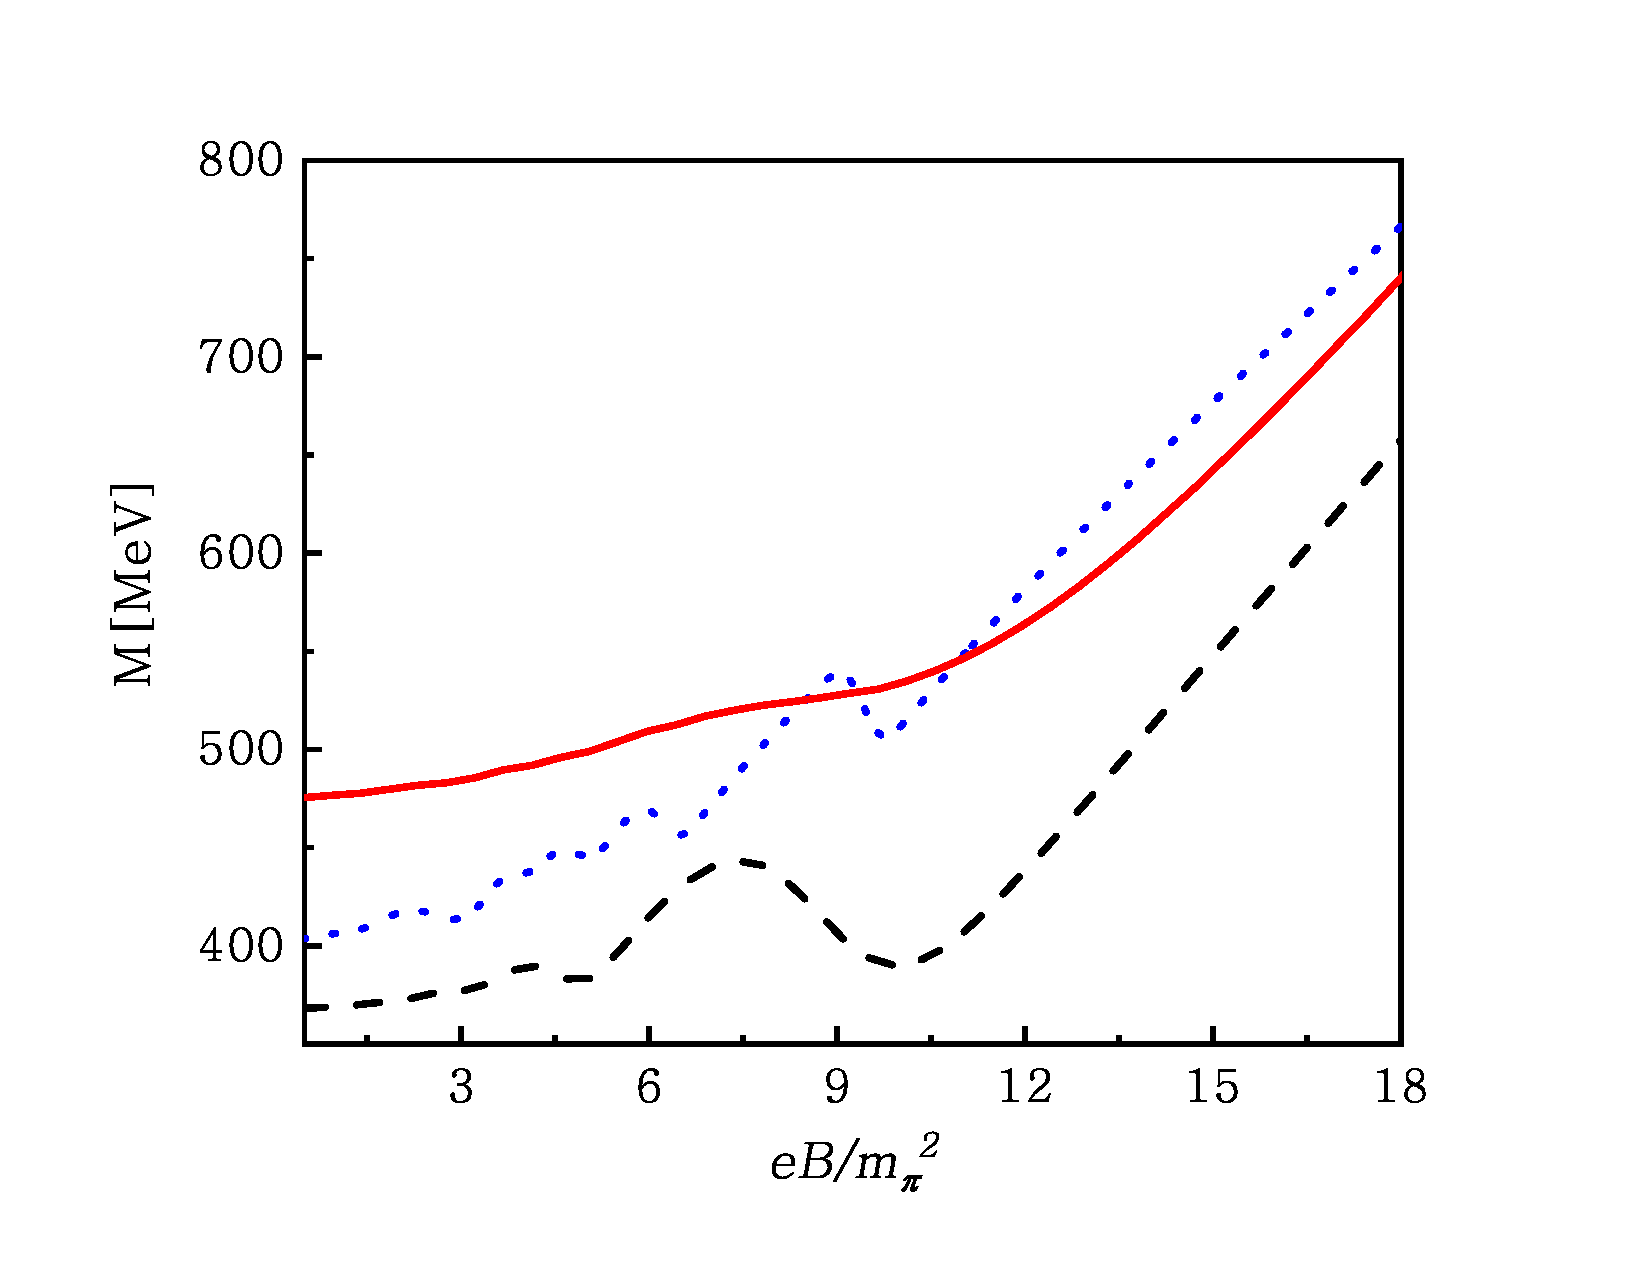
\includegraphics[scale=0.3]{compare.eps}
	\caption{Quark mass obtained by the Lorentzian function with $N=5$ (red solid line), $N=15$ (black dashed line) and Gaussian function (blue dotted line).}
	\label{f1}
\end{figure}

%To this end, it should be stressed that van Alphen-de Haas(vA-dH) oscillation happened in gaps (including $\Delta$, $\Delta_B$ and $M$) still exist.
%Recent study suggested a new regulator scheme named "Magnetic Field Independent Regularization"\cite{allen2015magnetized}.
%In Ref.\cite{allen2015magnetized}, the NJL-type model is investigated by using this regularization procedure in which the contributions that are explicitly dependent on the magnetic field turn out to be finite and do not required to be regularized. 
% the cutoff $\Lambda$ and the chiral coupling  $G$ is fixed by fitting the pion properties in vacuum, e.g.,
% the pion mass $m_\pi = 140$MeV and the constituent quark mass $M = 340$MeV.
% The diquark coupling constant $H$ is fixed by fitting the color superconductor gap.
% For the six-fermion coupling parameters $K$ and $K'$, one appropriate value of  $K'/K=4.2$\cite{abuki2010nambu} which satisfy the appearance of low-temperature critical phenomena.


\section{Numerical calculations and discussions}
\label{sec:3}

As the global minimum of the thermodynamic potential Eq.~\eqref{finaleq}, three of order parameters $s$, $s_B$ and $\chi$ should be determined by
\begin{equation}
\frac{\partial\Omega}{\partial s} =0,\quad 
\frac{\partial\Omega}{\partial s_B} =0,\quad 
\frac{\partial\Omega}{\partial \chi} =0,
\end{equation}
self-consistently. In the absence of magnetic field, as pointed out in Ref.\cite{abuki2010nambu},
the COE of chiral and diquark condensates manifests itself as a Bose-Einstein condensed phase of diquark ``molecules". 
In the presence of magnetic fields, we need to define various kinds of diquark phases due to the splitting of $s$ and $s_B$.
In this section, we will refer the Bose-Einstein condensed phase with $s_B\neq 0$ and $s=0$ as $\text{BEC}_\text{I}$ and the phase with $s\neq 0$ and $s_B = 0$ as $\text{BEC}_\text{II}$ respectively. Also, the ordinary BEC phase is possible where both $s$ and $s_B$ have non-vanishing values. 

\subsection{COE phase structure}
\label{sec:3a}

With the given magnetic field, we calculate the order parameters and thus three of gaps numerically. Fig.\ref{f2} is a typical result for not-very-strong magnetic fields.
%%%%and it displays the phase structure of COE    
%model parameters; magnetic field obtain at $eB=4.6m^2_\pi$. %1.40\times10^{19}G.
%%
At the quark chemical potential $\mu= \mu_c^I \simeq313$MeV, the gap $\Delta_B$ comes to appear and thus the $\text{BEC}_\text{I}$ phase occurs. Thereafter $\mu_c^I$ denotes the critical value for $\text{BEC}_\text{I}$ transition. 
While the COE phase manifests as $\text{BEC}_\text{I}$, $\Delta$ is not admitted to occur solely for $\mu>\mu_c^I $. As shown in Fig.\ref{f2}, $\text{BEC}$ occurs at $\mu \simeq327$MeV and terminates at the reference chemical potential $\mu_X \simeq350$MeV satisfying $M=\mu$~\cite{kitazawa2008bound}. In the vicinity of $\mu_X$, there exists a crossover from the $\text{BEC}$ phase to the $\text{BCS}$ phase of color superconducting quark matter.  
Similar as the case without magnetic fields~\cite{abuki2010nambu}, 
not merely the COE phase region exists but also the critical phenomena take place.
The difference from zero-field result is that $\text{BEC}_\text{I}$, preceding the $\text{BEC}$, is a new magnetic-induced phase.
Also, the value of quark mass in Fig.\ref{f2} is noticed to be larger than that given in Ref.\cite{abuki2010nambu}. It might be related with the magnetic catalysis as well as the smooth regularization used in the present work. 
%%%%%%%At $\mu =\mu_X\approx 350$MeV,,  occurs. the  between $\text{BEC}$ and $\text{BCS}$appear, 
%When $\mu$ equals to $350$MeV around in Fig.\ref{f2}, this point, denoted as reference critical point $\mu_X$, satisfy the condition that $M=\mu$ \cite{duarte2015bec}.In this point, the cross from $\text{BEC}$ phase to $\text{BCS}$ phase appear. 
%The result of Fig.\ref{f2} is basically same to the zero-field result. As shown , %For moderate magnetic case, Fig.\ref{f2} basically same to the zero-field result. 

\begin{figure}[ht]
	\centering
	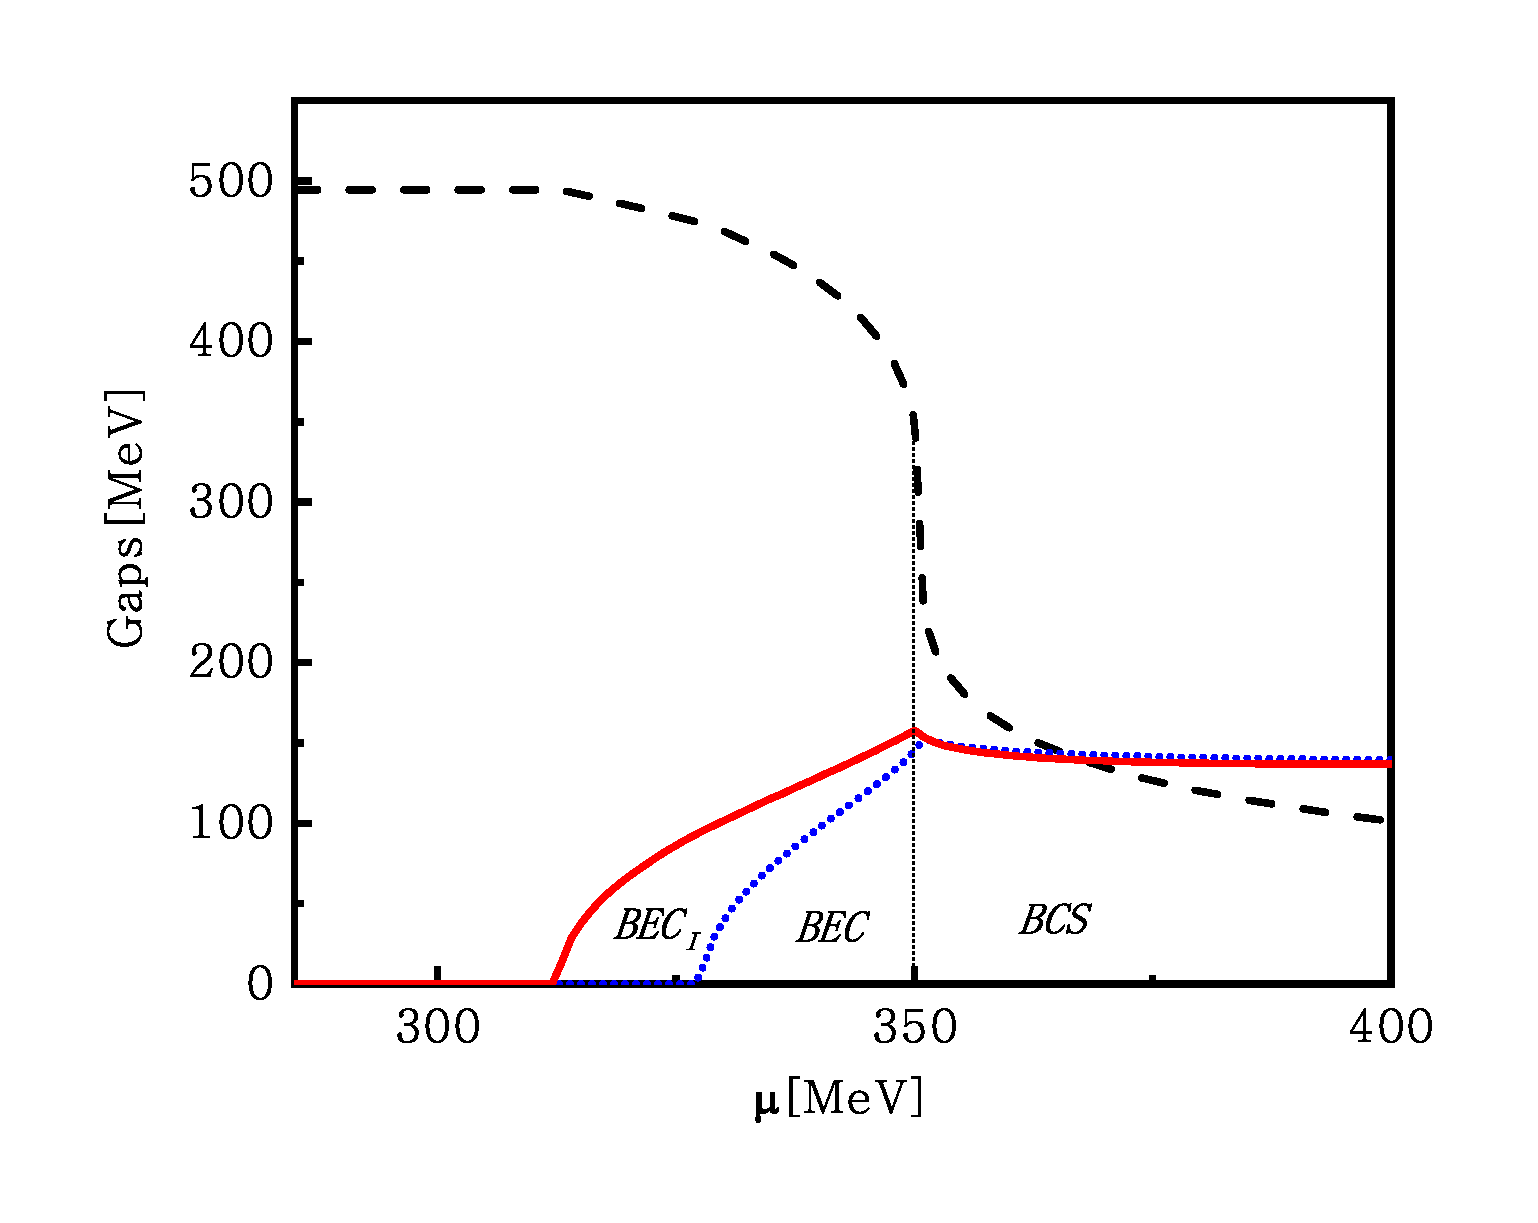
\includegraphics[scale=0.3]{1.eps}
	\caption{Constituent quark mass $M$ (dashed line), color-superconducting gaps $\Delta_B$ (blue dotted line) and $\Delta$ (red solid line) as functions of $\mu$ in the situation of $eB/m^2_\pi=4.6$.}
	\label{f2}
\end{figure}


With increasing magnetic filed, the COE phase structure changes gradually.
The whole region of COE is possible to be superseded by $\text{BEC}_\text{I}$. 
Numerical calculation shows that it happens as $eB$ approaches the threshold value.
% of magnetic field.
%%%%%
% corresponds to a , which will be discussed below.
%%have .the $\text{BEC}_\text{I}$ phase  occupies the whole COE region. In other words, the $\text{BEC}$ phase is suppressed by the strong magnetic field. As $\text{BEC}$ comes to be 
%%%%%%
Fig.\ref{f3} is a typical result for relatively large value of magnetic field. As shown in Fig.\ref{f3},
$\text{BEC}_\text{I}$ occurs at $\mu= \mu_c^I \simeq311$MeV and terminates at $\mu= \mu_X\simeq338$MeV.
In this case, $\text{BEC}$ is removed form the phase diagram completely. 
At around $\mu_c^I$ the quark mass remains continuous and it has no longer continuity at around $\mu_X$. As shown in Fig.\ref{f3}, indeed, there exist an obvious ``jump" of $M$ and some discontinuities of $\Delta$ and $\Delta_B$ at the reference chemical potential $\mu_X$. Thus, the critical phenomenon there is destroyed, which is the remarkable difference from zero-field result. 
%%%%%%
%change lies at t $\mu_X\simeq338$MeV, where the continuities of three gaps no longer take place.  
%For chiral phase transition, the second order transition predicted in zero-field case actually turns into a first order transition. 
%%%%%%%
%%

\begin{figure}[ht]
	\centering
	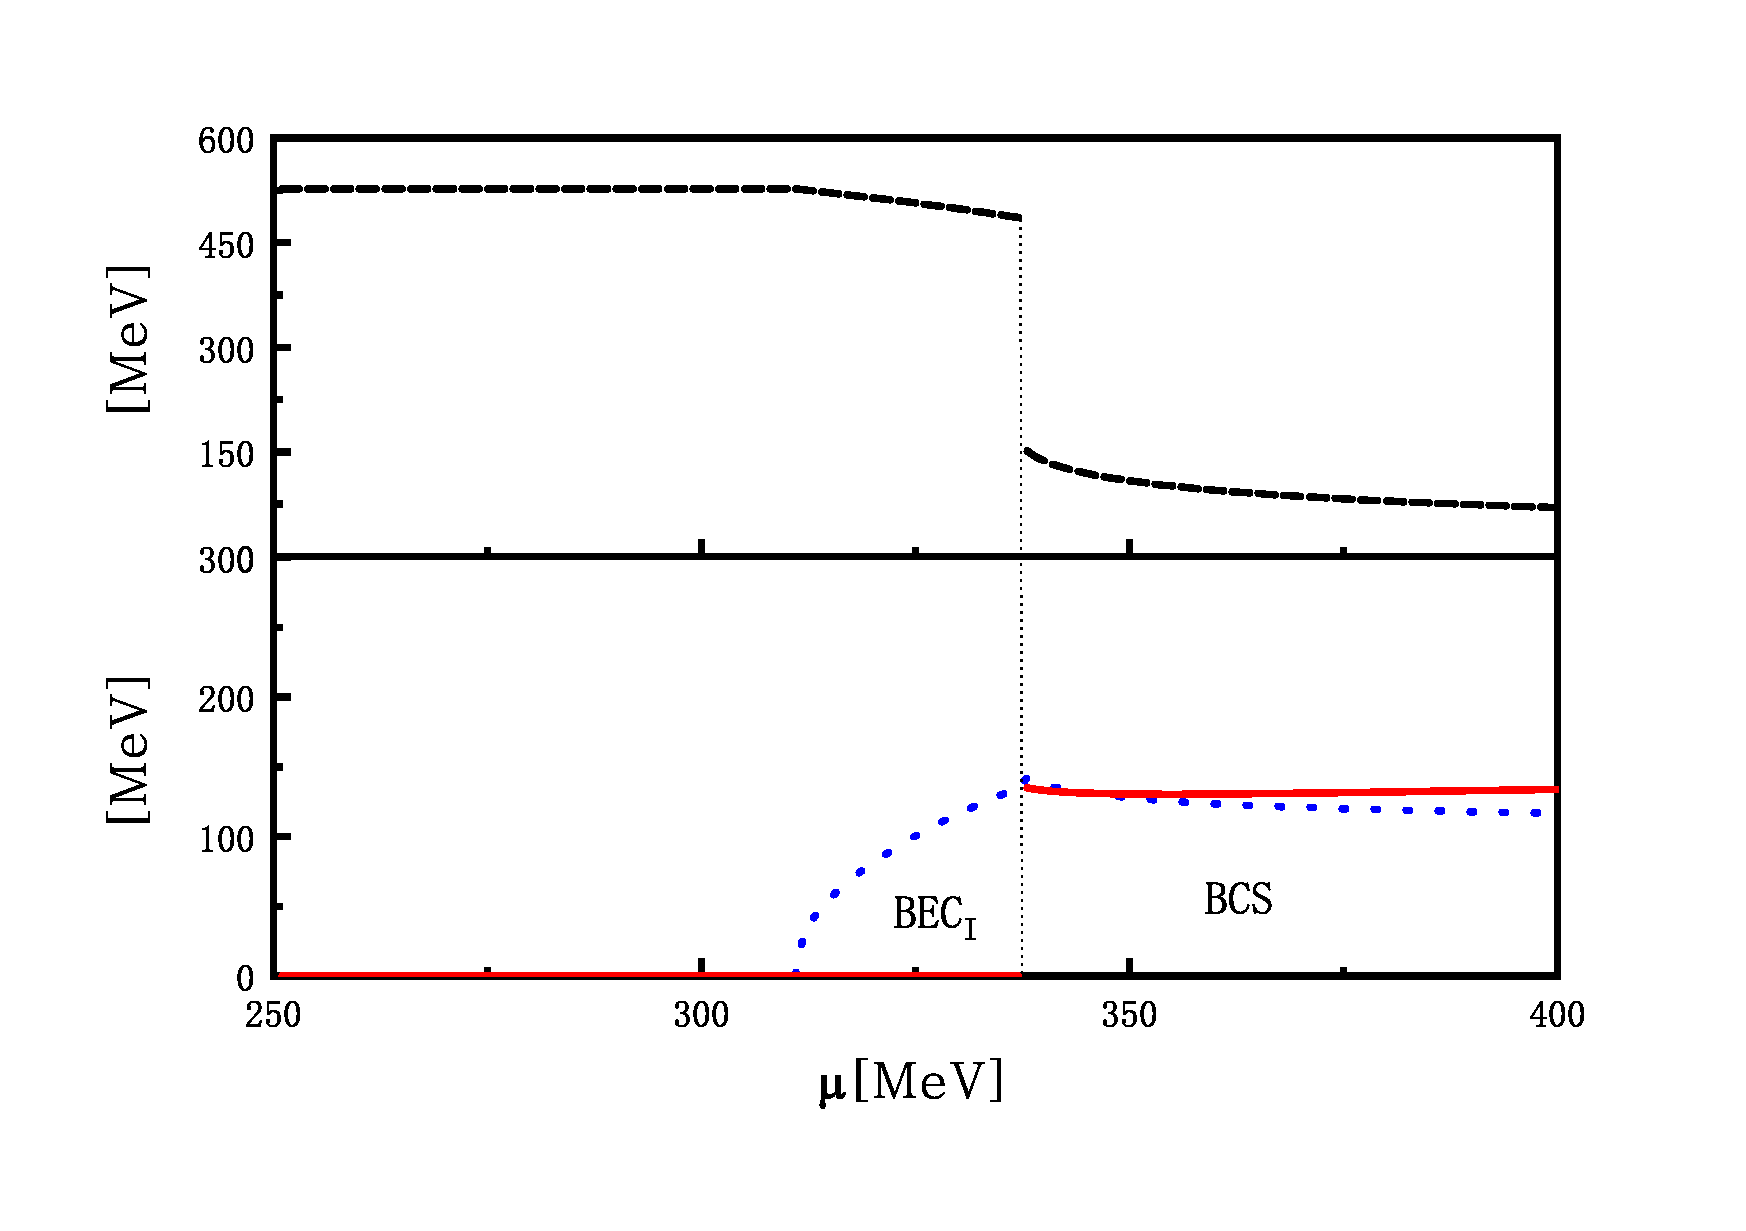
\includegraphics[scale=0.3]{92v2.eps}
	\caption{Similar as Fig.\ref{f2}, but $eB/m^2_\pi=9.2$.}
	\label{f3}
\end{figure}

\subsection{Criteria of Bose-Einstein condensed phases}
\label{sec:3b}

In order to understand the COE structure obtained above, we need to study the criteria of Bose-Einstein condensed phases.
For a designated phase with the effective coupling $H'$, its occurrence (as a second-order transition) is generally determined by~\cite{nishida2005bcs}
\begin{equation}
\label{eq:omegasecond}
 \frac{1}{H'}= Q(\vec{q} =0, \omega =0).
\end{equation}
In the absence of magnetic fields, the diquark polarization function $Q(\vec{q},\omega)$ has been derived from the 
one-loop contribution of quark propagator with three-momentum $\vec{p}$, see Ref.~\cite{abuki2010nambu} for details.
%%%%%%%%
%%With the effective coupling $H'$, the polarization function $Q(\vec{q},\omega)$ can be derived from the quark propagator with momentum $\vec{p}$. % 
At zero temperature the criterion of BEC transition reads
\begin{equation}
\label{eq:criticalfor1}
\frac{1}{H'} = \frac{8}{ \pi^2} \int_0^\Lambda\frac{ E p^2}{E^2 - \mu^2} dp.
\end{equation}
%%%%%%%
%\begin{equation}\label{eq:criticalfor0}
%  \frac{1}{4H'} =  4\sum_{\pm}\int \frac{d^3p}{(2\pi)^3} \frac{1-2f(E\pm \mu)}{2(E \pm \mu)}dp ,\end{equation}
%with the Fermi distribution function $f(\epsilon) =1/(e^{\epsilon/T} +1)$.
%%%where the Fermi distribution is $f(\epsilon) =1/(e^{\epsilon/T} +1)$ with $E=\sqrt{p^2+M^2}$ $E$ is the single-particle energy 
%  At zero temperature, Eq.~\eqref{eq:criticalfor0} has the form
%\begin{equation}\label{eq:criticalfor1}
%\frac{1}{H'} = \frac{8}{ \pi^2} \int_0^\Lambda\frac{ E p^2}{E^2 - \mu^2} dp,
%\end{equation}
%where the cutoff scheme is considered in Ref.\cite{abuki2010nambu}. 
%%%%%

In the presence of magnetic field, the splitting of diquark condensate leads to various kinds of Bose-Einstein condensed phases.
Let's firstly consider the case of $\text{BEC}_\text{II}$ transition. These quarks involved in the order parameter $s$ 
are (rotated-charge) neutral and thus no direct coupling to magnetic field exists.
%%%. occurrence $\text{BEC}_\text{II}$ involved order parameter    is $s$  and the paired   $s$  are always neutral.
%Thus there is no  direct coupling to magnetic field.  
Its criterion is easily obtained from
\begin{equation}
\label{eq:criticalforn}
\frac{1}{H'} =\frac{8}{ \pi^2} \int h_\Lambda  \frac{ E p^2}{E^2 - \mu^2} dp,
\end{equation}
which has the almost same form as Eq.~\eqref{eq:criticalfor1} unless the smooth regulator $h_\Lambda$ is introduced.
%By using Eq.~\eqref{eq:omegasecond}
%Compared with Eq.~\eqref{eq:criticalfor0}, the criterion equation of $\text{BEC}_\text{II}$ is formally equivalent with that obtained in the case of $B = 0$,Eq.~\eqref{eq:criticalforn} has the similar form as Eq.~\eqref{eq:criticalfor1}, except for
%excepted that we have introduced 
%the  diquark ``molecules"  are associated with

For $\text{BEC}_\text{I}$, the story is more complicated. Since the order parameter is $s_B$, as illustrated in Table.\ref{tab:1}, the involved components are not merely neutral quarks but also rotated charged quarks.
For the charged component, the single-particle energy corresponds to $E_B$ and the substitution such as Eq.~\eqref{eq:momentumsub} should be considered.
We take two kinds of contributions into account and then give the criterion of $\text{BEC}_\text{I}$ transition
\begin{equation}
\label{eq:criticalforq}
\frac{1}{H'}  =
 \frac{eB}{2\pi^2} \int \sum_{n=0}^{n_{max}} (1 -\frac{\delta_{n0}}{2}) h_{\Lambda, B}^n
\frac{E_B}{E_B^2 -\mu^2 } dp_3 + \frac{4}{ \pi^2} \int  h_{\Lambda}
\frac{Ep^2 }{E^2 - \mu^2} dp.
\end{equation}
While the second term is similar as Eq.~\eqref{eq:criticalforn}, the first term of R.H.S includes the direct coupling to magnetic field through the Landau level. 
In zero-field limit,  Eq.~\ref{eq:criticalforq} is recovered to the known result Eq.~\eqref{eq:criticalfor1}.
%%%%%that reflects the direct coupling of  rotated-charged quarks to magnetic field.
% Eq.~\eqref{eq:criticalforn}.
%%%%%%% 
In fact, these criteria may be considered from the alternative point of view. 
Regarding the thermodynamic potential as a Ginzburg-Landau expansion of $\Delta$ and $\Delta_B$,
the $\text{BEC}_\text{II}$ and $\text{BEC}_\text{I}$ transitions are given by vanishing coefficients of quadratic terms, i.e.\begin{equation}
  \frac{\partial^2\Omega}{\partial \Delta^2}|_{\Delta_B =0,\Delta =0} =0 ,\frac{\partial^2\Omega}{\partial \Delta_{B}^2}|_{\Delta_B =0,\Delta =0} =0,
\end{equation}
respectively. It is easily proven that the above equation can yield the results ~\eqref{eq:criticalforn} and ~\eqref{eq:criticalforq} equivalently. 


\begin{figure}[h]
  \caption{Critical chemical potentials $\mu_c^\text{I}$ (red solid line), $\mu_c^\text{II}$ (green dashed line), $\mu_c$ for BEC  (blue dashed dotted line)  and reference chemical potential $\mu_X$ (black dotted line).}
  \centering
    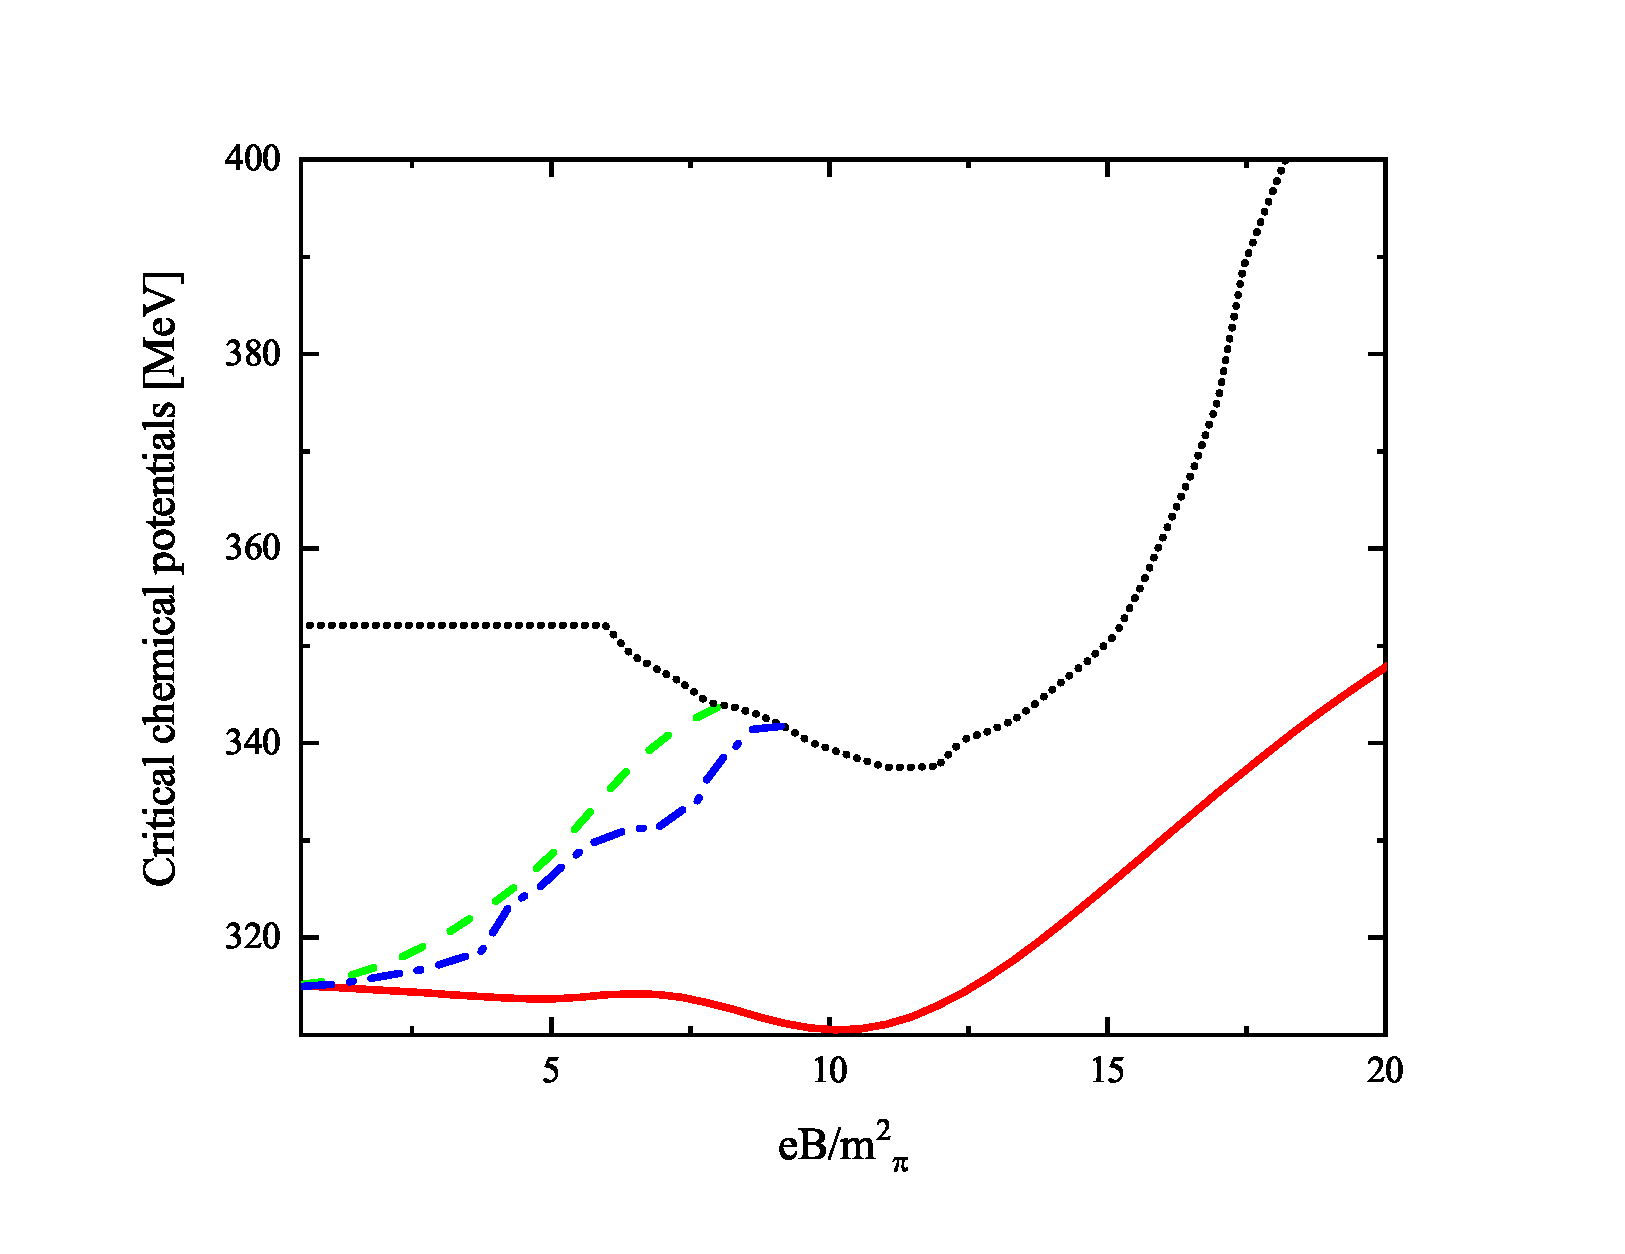
\includegraphics[width=0.6\textwidth]{third.eps}
    \label{fig:thirdpoint}
\end{figure}

By using Eqs.~\eqref{eq:criticalforn} and ~\eqref{eq:criticalforq}, we give the critical values for Bose-Einstein condensed phases and their magnetic-field dependence in Fig.\ref{fig:thirdpoint}.
With introducing magnetic field, firstly, the value of $\mu_c^\text{I}$ comes to be less than  $\mu_c^\text{II}$ or $\mu_c$. It explains why the $\text{BEC}_\text{I}$ occurrence exceeds other phases, say $\text{BEC}_\text{II}$ and $\text{BEC}$.
If $\text{BEC}_\text{II}$ existed, it would have the position for $eB \lesssim  8 m_\pi^2$, at which the line of $\mu_c^\text{II}$ meets that of $\mu_X$. In this regime, as has been observed in Figs.\ref{f2} and \ref{f3}, there actually exist either $\text{BEC}_\text{I}$ or $\text{BEC}$.
%%%%%%%
%% $\text{BEC}_\text{II}$ does not appear in the phase diagram. 
As shown in Fig.\ref{fig:thirdpoint}, secondly, $\text{BEC}$ exists 
until $eB \approx 9m_\pi^2$ at which $\mu_c$ meets $\mu_X$.
It corresponds to the above-mentioned threshold value of magnetic field.
For fields larger than this threshold, $\text{BEC}$ does not appear in the phase diagram yet.
In this regime, $\mu_c^\text{I}$ is less than $\mu_X$ and no intersection of two lines is found. It explains why $\text{BEC}_\text{I}$ remains to be the COE phase throughout. 
%%%as shown in Fig.\ref{f3},  the BEC phase  appears only forintermediate magnetic  field.
%for intermediate magnetic field, there is the position of the so-called BEC phase.Actually, the BEC phase exists for intermediate $B$ field
%and is removed from the phase diagram with the increasing $B$ field.
%%At $eB \simeq 8 m_\pi^2$,  $\text{BEC}_\text{II}$ phase disappears since the crossover to BCS phase has happened. In fact,
%there exist no possibility for  the imaginary $\text{BEC}_\text{II}$ phase with zero value of diquark condensate $s_B$, owing to   non-zero value of diquark condensate $s_B$ raises firstly.
%Therefore BEC phase with non-zero value of diquark condensates $s$ and $s_B$ appears in the phase diagram.
%This fact could explain the result shown in the phase diagram Fig.\ref{f3}.
%Finally, at $eB > 10 m_\pi^2$,
%the location of $\mu^{I}_c$ shifts  to relatively larger chemical potential  and $\mu^{I}_c$  is always smaller than  $\mu_X$.
%Therefore the  $\text{BEC}_\text{I}$ phase exists still in the phase diagram.tendencies.

Also it is observed that, for intermediate magnetic fields, the various critical chemical potentials have different tendencies.
While the critical values for $\text{BEC}$ and $\text{BEC}_\text{II}$ are almost the increasing functions of $eB$,
$\mu_c^\text{I}$ behaves as a decreasing function in the regime of $6 m_\pi^2 <eB < 10 m_\pi^2$.
It is important to notice that, as COE of chiral and diquark condensates, the $\text{BEC}_\text{I}$ occurrence corresponds to the critical end point of chiral phase transition.
The decreasing tendency of $\mu_c^\text{I}$ means that, with increasing magnetic field, chiral transition occur at lower chemical potentials. It contradicts the known magnetic catalysis, namely the critical value for chiral transition increases with increasing field, see, e.g.~\cite{Gusynin1994Dimensional,Miransky2012Catalysis}. In this sense, the phenomenon could be regarded as inverse magnetic catalysis.
%%%%%
%magnetic-field-dependence. monotonic%For , $\mu_c^\text{II}$  behaves as an increasing function .  is not a  increasing function, at least   regime.%%%%critical phenomena appears  and $\mu_c^\text{I}$ can be understood as  ,
%Owing to this inverse magnetic catalysis effect,  $\mu_c^\text{I}$ is always less than $\mu_X$. 
%% the value of BEC-BCS crossover
%In this sense, the IMC happened in $T=0$ and intermediate value of magnetic field is responsible for the result in phase diagram.
The inverse catalysis originate from the coupling of rotated-charged quarks to magnetic field in the result of $\mu^\text{I}_c$, rather than oscillations of gaps, say the oscillating quark mass. Even though nonphysical oscillation is removed as much as possible, as stressed in Ref.\cite{duarte2015bec}, the inverse catalysis holds valid for intermediate fields and zero temperature. 
%%%%%%%
%. In the situation with intermediate magnetic fieldsthere exist oscillating behaviors. But it is not the main reason for . %conclusion of inverse catalysiscan still  be drawn, .%%% decreases i%For $\mu_X$, there existThe possible oscillation 


\subsection{Strong  field analysis for  \texorpdfstring{$\text{BEC}_\text{I}$}{Lg} }
\label{sec:3c}

In strong field limit where the lowest Landau level works, a simple argument is usually accessible.
For the chiral broken phase (the phase with $\chi \neq 0$ only), 
the magnetic effect becomes important as the magnitude of $eB$ reaches the scale of $m_\pi^2$.
In the experiments of heavy-ion collision, for instance, the strong field is estimated to be 
$eB \approx 15 m_\pi^2$, see,e.g.~\cite{V2009ESTIMATE}.
%%%%% As a typical example, the strong  fields  are observed to have magnitudes of the order $eB \approx 15 m_\pi^2$
%\cite{V2009ESTIMATE}.
For the BCS phase of magnetized CFL matter, as pointed out in \cite{ferrer2005magnetic},
the strong field is estimated to be $eB \approx \mu^2$.
%%%%%% (the magnetized CFL phase considered in literatures),
%the relevant scale for the generation of the diquark gaps is  the quark chemical potential.
%Once the magnitude of the magnetic field is comparable to the chemical potential, i.e. $eB \sim \mu^2$, 
%$\mu^2$ is used as the system of the magnetic  field scale. the value of magnetic field reaches to $\mu^2$, and then
 %the difference between $\Delta$ and $\Delta_B$ gaps  becomes significant
%% the density of states on the Fermi surfaceof the charged quarks will be larger thanthat of neutral quarks.
For our concerned $\text{BEC}_\text{I}$ phase, the so-called strong field might be estimated by a simplified form of the criterion Eq.~\eqref{eq:criticalforq}.
%%%%%%  is simplified as follows. 

Because of the dimension reduction,
the first term in Eq.~\eqref{eq:criticalforq} becomes
\begin{equation}\label{eq:cond2}
 \frac{eB}{ 2\pi^2} \int h_{\Lambda,B}^{n=0}
\frac{ \sqrt{p_3^2 + M^2}}{p_3^2 + M^2 - \mu^2} dp_3,
\end{equation}
and the criterion for $\text{BEC}_\text{I}$ is reducible 
\begin{equation}\label{eq:cond3}
  \frac{1}{H'} =  \frac{eB}{2\pi^2} \int^\Lambda_0\frac{E}{E^2-\mu^2}dp
  +\frac{4}{\pi^2}\int^\Lambda_0 \frac{E}{E^2-\mu^2} p^2 dp,
\end{equation}
in the strong field limit. There the usual single-particle energy $E$ and the hard cutoff have been used.
By using Eq.~\eqref{eq:cond3}, it is found that $\mu^{I}_c$ increases with $eB$ monotonically. Compared with the result of Fig.\ref{fig:thirdpoint}, we find that Eq.~\eqref{eq:cond3} becomes valid at least for $eB \gtrsim 11 m_\pi^2$. It corresponds to the strong field in our numerical calculations.

%%%%%%This tendency has been observed in Fig.\ref{fig:thirdpoint} for strong fields.    
\begin{figure}[h]
  \caption{ Ratio of effective diquark coupling required for $\text{BEC}_\text{I}$ transition in strong field limit. }
  \centering
    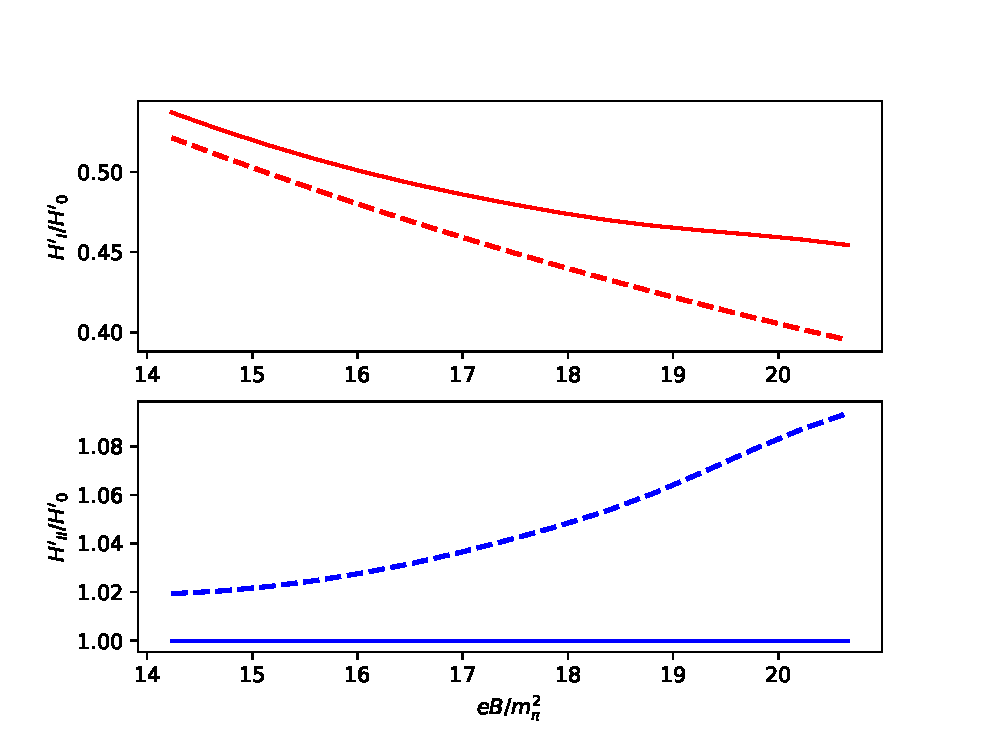
\includegraphics[width=0.5\textwidth]{h.eps}
    \label{fig:h}
\end{figure}
%%% Solid line denotes ratio of the effective coupling required for $\text{BEC}_\text{I}$  in strong field limit. Dashed line has ignored the magnetic effect from $M$. }%

By applying Eq.~\eqref{eq:cond3}, it is interesting to investigate how
the QCD axial anomaly varies as $\text{BEC}_\text{I}$ occurs. As well known, the anomaly leads to the chiral-diquark interplay $K'$ and makes the diquark coupling become effective $H' = H -\frac{1}{4}K'\chi$~\cite{abuki2010nambu}. 
For the illustrative purpose, we firstly consider the case of effective coupling $H'$.
In Fig.\ref{fig:h}, its magnetic-field dependence is given for the given quark chemical potential $\mu=315$MeV.
We have normalized the coupling $H'$ with respect to its zero-field result $H'_0$.
As depicted by the solid line, it manifests a monotonic decreasing function.
This indicates that, with increasing magnetic field, the smaller strength of $H'$ is required for $\text{BEC}_\text{I}$ transition.
In other words, strong fields actually facilitate the $\text{BEC}_\text{I}$ occurrence.
Analytically, this result stems from the direct coupling to $eB$ as well as the implicit $eB$-dependence of quark mass, which plays the role through the single-particle energy $E$ (see Eq.~\eqref{eq:cond3}).
%%%%%%%%%%%
%an explicit coupling to $eB$ (i.e., the first term of Eq.~\eqref{eq:cond3}).
%In fact, the behavior of $H'_{I}$ depends on the effect for  $eB$ relevant term as well as magnetic catalysis effect  from
% the effective mass $M$.%  we can give the magnetic field behavior of $H'$ by
%  incorporating  $M$  into Eq.~\eqref{eq:cond3} 
%Besides, the strong field result of $H'$ origniates from an implicit $B$-dependence of $E$, exactly the dependence of quark mass.
%Interestingly,
Note that the latter dependence of quark mass displays
a monotonic increasing function, i.e. the magnetic catalysis for strong fields.
%%~\cite{Gusynin1994Dimensional,Miransky2012Catalysis}.
If ignoring such magnetic catalysis, $H'$ would be a more obvious decreasing function of $eB$. This tendency is shown by the dashed line of Fig.\ref{fig:h}. 
For the qualified coupling $H'$ to achieve $\text{BEC}_\text{I}$, therefore, the magnetic effect on chiral condensate
cancels out the effect on rotated-charge relevant diquark condensate partly.
%%%%
%It is clear in Fig.\ref{fig:h} that the magnetic effect caused by the $eB$ coupling is partial compensated that the magnetic  effect from $M$.


\begin{figure}[h]
\caption{Phase diagram in the $\mu$-$K'$ plane in strong-field limit.
Thick (red) solid line denotes the first-order chiral transition, thin (green) solid line is $\text{BEC}_\text{I}$
transition and dotted (blue) line is a crossover between $\text{BEC}_\text{I}$ and $\text{BCS}$.}
\centering
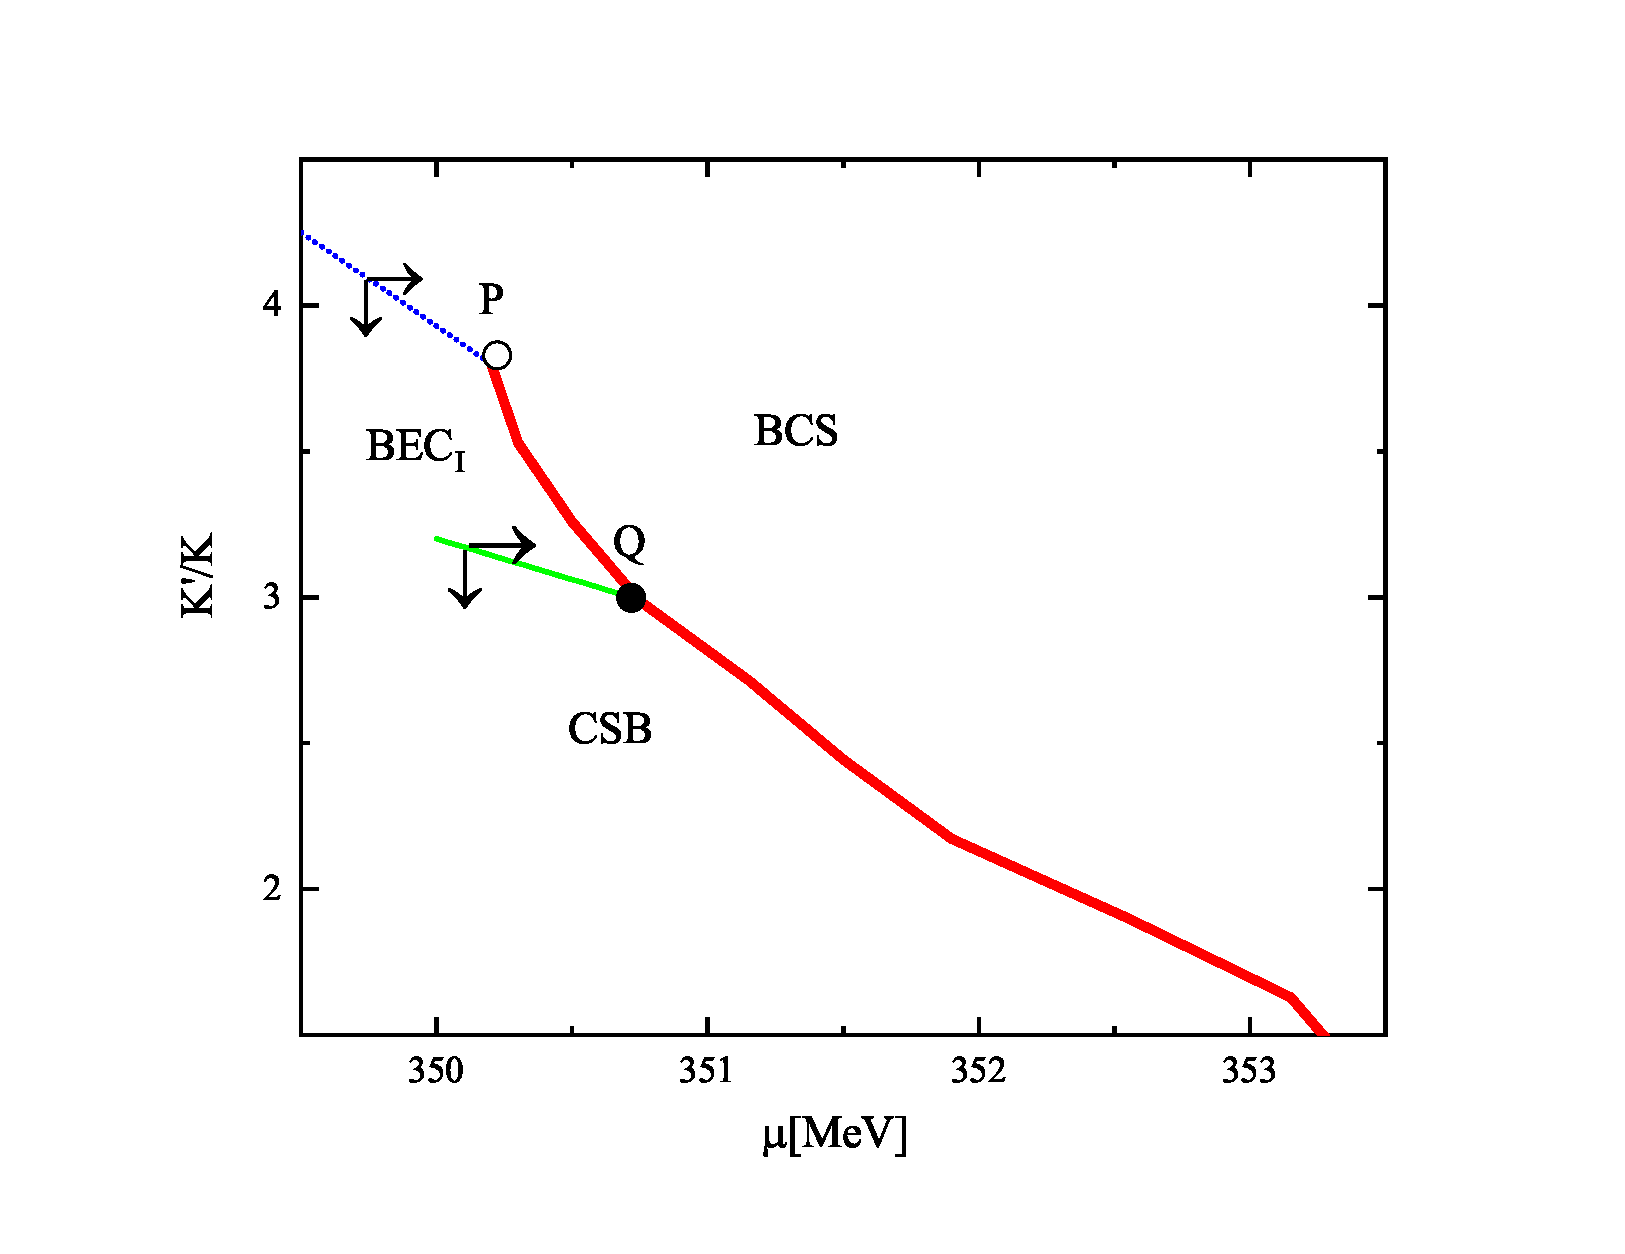
\includegraphics[width=0.6\textwidth]{kmu.eps}
\label{fig:kmu}
\end{figure}

Then, we consider the case of chiral-diquark interplay $K'$.
In Fig.\ref{fig:kmu}, the phase diagram in the $\mu$-$K'$ plane is plotted at the given strong field. 
For small strength of $K'$, the chiral symmetry broken phase (CSB) and the BCS phase are separated by a first-order chiral transition (red, thick solid line).
Once the qualified $K'$ is chosen, a second-order phase transition from CSB to 
$\text{BEC}_\text{I}$ takes place (green, thin solid line). As expected, the COE of chiral and diquark condensates appears in the phase diagram. With increasing $K'$, the COE phase ($\text{BEC}_\text{I}$) might be terminated by the crossover (blue, dotted line). The phase diagram is basically similar as the zero-field result, namely Fig.9 of Ref.~\cite{abuki2010nambu}.
On the other hand, there exist two of intersection points in Fig.\ref{fig:kmu}. As the intersection of $\text{BEC}_\text{I}$ and chiral transitions, the point Q behaves as a critical end point of chiral transition. In the vicinity of $Q$, the order parameters have been observed to be continuous.
As for the intersection point $P$ of chiral transition and $\text{BEC}_\text{I}$-BCS crossover, it is not a critical point since  
critical phenomenon no longer happens there. In this sense, the characteristic of intersection point is different from the zero-field case.
%%%%%%%%
% (see, e.g. Fig.9 of Ref.~\cite{abuki2010nambu}). 
%%%
%obtains the required value for Eq.\eqref{eq:cond3},
%%%%: the thin solid line meets the thick solid line at  point $Q$ and the dotted line meets the thick solid line at point $P$.
% In the  vicinity of point $P$, in Fig.\ref{f3}, the order parameter $M$ is discontinuous 
%the intersection point of chiral phase transition and crossover to  lines,

Finally, let us discuss the magnetic-induced evolution of $\text{BEC}_\text{I}$ qualitatively.
In the situation with a given parameter $K'$ and increasing magnetic field, as shown by the horizontal arrows in Fig.\ref{fig:kmu},
both the $\text{BEC}_\text{I}$ transition and the $\text{BEC}_\text{I}$-$\text{BCS}$ crossover move towards 
larger quark chemical potentials.
It indicates that strong fields make the $\text{BEC}_\text{I}$ phase to be located at reasonably high baryon densities.
%%%%%%%
% the thin solid line  and  dotted line shift to  larger chemical potentials with increasing magnetic field.
% This tendencies  are shown by the horizontal arrows  in Fig.\ref{fig:kmu}. It indicates that strong fields make the location of $\text{BEC}_\text{I}$ moves towards   higher densities in phase diagram.%%%
%in  $K'$-$\mu$ phase diagram 
%%%%%%%%%%
In the situation with given $\mu$, on the other hand, the two of lines move towards smaller strength of $K'$, as shown by the vertical arrows. Obviously, this tendency is consistent with that of $H'$ given in Fig.\ref{fig:h}. It indicates that the qualified chiral-diquark interplay is suppressed by strong magnetic fields.
%%%%%%%%%%%%%%%
%to achieve $\text{BEC}_\text{I}$existence of strong fields makes   required become weaker.
%smaller strengths of QCD axial anomaly with increasing magnetic field.



\section{Conclusion and outlook}
\label{sec:4}

In this work we investigate coexistence of chiral and diquark condensates and moderate-density and zero-temperature critical phenomenon in the presence of magnetic fields. Generally, critical phenomena depend on the symmetries and symmetry breaking patterns of order parameters.
%%%%%
%In the absence of magnetic fields, the model-independent analyses had been given for the critical phenomenon~\cite{yamamoto2007phase,hatsuda2006new}.
%%\cite{hatsuda2006new},%%%%%%%%%%%%%%
The color-flavor locked breaking pattern is 
 $SU(3)_C \times SU(3)_L \times SU(3)_R \times U(1)_B \times U(1)_A \rightarrow SU(3)_{C+L+R}$. Within a Ginzburg-Landau (GL) framework, diquark condensate is described by a $3\times 3$ matrix, say $d_L=-d_R=\text{diag}(s,s,s)$, and chiral condensate is described by $\Phi=\text{diag}(\chi,\chi,\chi)$~\cite{yamamoto2007phase,hatsuda2006new}.  
In the absence of magnetic fields, the axial anomaly yields cubic terms, say $s^2 \chi$, in the GL free energy and the chiral-diquark interplay leads to the critical phenomenon in the phase diagram.
Once strong magnetic fields are introduced, the symmetry is further broken to $SU(2)_{C+L+R}$\cite{ferrer2006color}.
%%%%%%%%%%%%%
% and the magnetized CFL matter appears at high densities.
%%%%%%%%%%%%%
%eaking pattern becomes$SU(3)_C \times SU(2)_L \times SU(2)_R \times U(1)_B \times U(1)_A \rightarrow  SU(2)_{C+L+R}$
%in the absence of magnetic fields.
%%%%%%%%
A similar analysis might be valid for the $\text{BEC}_\text{I}$ phase. While the matrix $\Phi$ holds unchanged, the diquark condensate matrix becomes $d_L=-d_R=\text{diag}(0,s_B,s_B)$ formally. In this case, there exists the term like $s_B^2 \chi$.
Thus, strong magnetic field does not preclude the axial-anomaly induced critical phenomenon. 
%%%%%%%%%%%%%%%
%%with non-vanishing $s_B$ and $\chi$. 
%the axial anomaly such as $d_R d_L^\dagger \Phi$ still yields some of cubic terms, say the chiral-diquark interplay . It means that %%%From our results, for instance, the point $Q$ in Fig.\ref{fig:kmu} corresponds to the critical end point of chiral transition and the critical phenomenon still takes place around it.
%%% %%%%%%%%%%%%%%%%%%%%%%%%%%%%
However, it is difficult to proceed a complete GL analysis. While diquark condensate
becomes split, the rotated electromagnetic field needs to be incorporated and possible rotation between $d_L$ and $d_R$ should be considered. Also the qualitative GL analysis could not explain COE and the associated critical phenomena, unless these microscopic details are known.
%%%%%%%%
%%%At least for the phenomenon regarding for the situation with non-zero $s$, $s_B$ and $\chi$.
%Due to the magnetic-induced splitting, the diquark-condensate matrix decomposes into two parts, namely the part relevant to $\frac{1}{3}(s+ 2s_B)$ and that relevant to $\text{diag}(\frac{2}{3}, -\frac{1}{3},-\frac{1}{3})$. 
%%%%
%Now that electric charge matrix emerges in the latter, the electromagnetic field needs to be incorporated into the GL free energy. Also, the possible rotation between $d_L$ and $d_R$ need to be considered. 
%%%%%%
%%%%%%%%%%%%%%%%%%%%%%%

The quantitative discussion of magnetic influences is the content of the present work.  
In a phenomenological NJL model with axial anomaly, we derive the formalism of magnetized CFL matter and the criteria of different Bose-Einstein Condensed phases. Besides the complicated phase structure, our attention is mainly paid to the $\text{BEC}_\text{I}$ occurrence. For various strengths of magnetic field, we briefly discuss several implications of our main results.
\begin{enumerate}[(i)]

\item The inverse magnetic catalysis (IMC) is observed for intermediate fields, say $ 6m_\pi^2<eB < 10m_\pi^2$ according to our numerical calculations. This phenomenon has been widely predicted from the high-temperature Lattice QCD to the model studies in zero temperature case~\cite{andersen2016phase,duarte2015bec}.
%%%%%ADD:: highT IMC Refs???%%%%%%%%%%%%
In two-color and two-flavor NJL model without axial anomaly, the quarks with rotated electric charges $\pm \frac{1}{2}$ were considered in Ref.\cite{duarte2015bec}. As the COE phase, the resulting Bose-Einstein Condensed phase is similar as the present-discussed $\text{BEC}_\text{I}$. It is not surprising then that our result of IMC has analogy to the case of Ref.\cite{duarte2015bec}.  
%%%%%%
%)  the critical value of $\mu^{I}_c$ as functions of $eB$ has a decreasing tendency. Such tendency can be understood as IMC. Ieven though t was not considered there.Since the  phenomena are found in both cases, the IMC effect might be the basic feature of OCD in the presence of intermediate magnetic fields. 
%%%%%%%%%%%%%


\item The role of strong fields that facilitate the $\text{BEC}_\text{I}$ occurrence is clarified by arguments in the lowest Landau-level limit. For the fields $eB > 11m_\pi^2$, its critical value $\mu^\text{I}_c$ is observed to increase monotonically. Stronger fields mean that $\text{BEC}_\text{I}$ (as the COE phase) is located at larger quark chemical potentials and/or higher baryon densities.
%%%%%%
%as well as the critical chemical potential $\mu_X$ are found 
%%%%%%%%%%
%%location pushed to $\text{BEC}_\text{I}$ is found at relatively large chemical potential.
%For stronger magnetic fields, we observe that   coupling of the chiral-diquark interplay and its  is   
%%%%%%%%%%%%%%%
At the same time, it requires smaller strengths of the chiral-diquark coupling $K'$ and/or smaller strengths of the effective coupling $H'$. Note that the QCD axial anomaly is believed to become suppressed in high-density quark matter, see,e.g.~\cite{T2002Instanton,R2000High}. By introducing strong fields, therefore, $\text{BEC}_\text{I}$ and the COE phase region are updated to exist in more realistic situation and/or more reasonable physical environment. 

This theoretical prediction could have potentially importance for astrophysics, since $eB\simeq 11m_\pi^2 \sim10^{20}\text{G}$ discussed here reaches the estimated value for interior field in magnetars~\cite{lai1991cold}. Taking the $\text{BCS}$ phase of magnetized CFL matter into account, stellar models of hybrid stars with quark core and self-bound quark stars had been studied in recent years, see, e.g. Refs.\cite{ferrer2013magnetism,paulucci2011equation}. 
If $\text{BEC}_\text{I}$ exists and constitutes the interiors, it is likely that stellar models of mixed stars with the core of COE
(without sharp interface) would be needed. Also, such kind of possibility might represent a new open opportunity for exploring the 
the continuity between chiral-broken matter and color superconducting matter.

\end{enumerate}
%%%%%%%%%%%%%%
%, t the situation with strong field corresponds to a more .
%%%In other words,  when a relatively small axial anomaly coupling is chose.
%%% required for $\text{BEC}_\text{I}$ transition are found to be pushed torelatively small for strong field.
%%magnetic-field dependences of As depicted in Fig.\ref{fig:kmu}, 
%%Noticing that the QCD axial anomaly caused by instanton effects would be suppressed at high densities\cite{T2002Instanton,R2000High}
%%%% understanding the physical realization of dense matter.
%%%the  of r, would be further studied in future.
%%%%%%%%%%%%%%%%%%%%%%the physics of magnetars%
%There the surface magnetic field has the order of $10^{14}$-$10^{16}$G~\cite{bogomazov2007evolution,mereghetti2015magnetars:}.In the interior region, the s of maximum fields are large as $10^{18}$-$~\cite{paulucci2011equation}.
%%%%%%%%%%%%
%%%%%%%%%
%%  %%%%%%%%%%%%
%physics, on the other hand,  a common characteristic of compact stars is their strong magnetization.I,  %%%%%%%%%%

The present study is based on a minimal extension of the NJL model with axial anomaly.
In more realistic NJL models where multiple flavors with bare masses, effect of confinement, color neutrality and so on are considered,
the resultant phase structure becomes more and more complicated unavoidably, see, e.g.~\cite{basler2010role,Powell2011Axial,powell2013asymmetric}. 
%%%%%%%%%%%%% 
%%%the first step for exploring magnetic effects on the diquark-chiral condensate coexistence.such physical elements  
%%%% quark bare masses might lead to a rich phase structure% shows that two-flavor superconducting pairing could be favored owe to spontaneous flavor-symmetry breaking caused by the axial anomaly and this would .It would be interesting to  investigate open problems include whether the two-flavor color superconducting pairing  would survive in COE region and how the  phase structure changes with magnetic fields.%%%%%%and the Polyakov loop term describing the de-confinement transition could give rise the asymmetric CFL phase~\cite{Powell2013Asymmetric}.
%%%%%%% the color neutrality by restricting ourselves to a single quark chemical potential. A rigorous investigation for realistic quark matter should be included the effect from  color neutrality.
%%%%%%%%%%%%
In the presence of magnetic fields, not merely splitting of diquark condensate but also ``splitting" of the longitudinal and transverse pressures are important for applications of CFL matter. The latter was taken into account in Ref.\cite{paulucci2011equation}, but 
has not been considered in the present work. 
Also, there are alternative smooth regularization schemes in the studies of magnetized matter with diquark condensate. 
For instance, the scheme called magnetic field independent regularization was adopted to remove nonphysical oscillations of gaps~\cite{duarte2015bec,coppola2017magnetized}.
Towards further studies of our presented $\text{BEC}_\text{I}$ and its applications inside magnetars, we will discuss these problems listed above in a future publication.
%%%%%%%%%%%%being elucidated in future.%%%%
%calculating equation of state of dense matter.where  as well as the separation 
%In this way, a clearer interpretation of the physical oscillations is possible.How to generalize this  regularization scheme  to the case of three-flavor NJL model with axial anomaly is still open question.
%%%%%%Finally, the crossover between diquark Bose-Einstein Condensed phase(s) and BCS phase . For the latter, a relativistic %crossover had been discussed in the presence of magnetic fieldsee, e.g.~\cite{wang2011magnetic}.
%%%%%%%%%%%%%%%%

\begin{acknowledgements} 
The authors  thank  Hui Wang  for  technical assistance, comments  and suggestions.
This work was supported by National Natural Science Foundation of
China ( NSFC ) under Contract No. 10875058.
\end{acknowledgements}

%\bibliographystyle{apsrev4}
\bibliographystyle{unsrtnat}
\bibliography{bib1}

\end{document}


\end{document}

